% !TeX program = lualatex
\documentclass[11pt,a4paper]{article}
\usepackage{szzmaterial}
% Strojopis = DejaVu Sans Mono: má všechny řezy (regular/bold/italic) i plnou
% českou sadu s PŘEDKOMPONOVANÝMI glyfy (Libertinus Mono nemá ů/ě/ř s háčkem
% předkomponované -> accent se ve výpisech odtrhne). MatchLowercase srovná velikost.
\setmonofont{DejaVu Sans Mono}[Scale=MatchLowercase]
% Umožní psát `_` jako podtržítko v běžném textu i v komentářích výpisů (texcl).
\usepackage[strings]{underscore}
\usepackage{tikz}
\usetikzlibrary{positioning,arrows.meta,calc,fit,backgrounds,shapes.geometric,shapes.misc,matrix}
\setlist[enumerate]{nosep,leftmargin=2.1em}
\setlist[itemize]{nosep,leftmargin=1.8em}

% --- Styl výpisů C++ (lokální doplněk preambule okruhu) ---
\lstdefinestyle{cpp}{%
  language=C++,
  basicstyle=\ttfamily\footnotesize,
  keywordstyle=\color{blue!60!black}\bfseries,
  commentstyle=\color{green!40!black}\itshape,
  stringstyle=\color{purple!70!black},
  showstringspaces=false,
  columns=fullflexible,
  keepspaces=true,
  breaklines=true,
  breakatwhitespace=true,
  frame=single,
  framerule=0.4pt,
  rulecolor=\color{black!30},
  backgroundcolor=\color{blue!2},
  xleftmargin=5pt,xrightmargin=3pt,
  aboveskip=5pt,belowskip=3pt,
  tabsize=2,
  morekeywords={override,final,noexcept,constexpr,nullptr,decltype,
    co_await,co_return,concept,requires,thread_local,alignas},
  % Diakritika: listings zpracovává vstup po BYTECH a znaky Latin Extended-A
  % (ě ř č ž š ů ...) přehazuje. texcl=true sází obsah řádkových komentářů jako
  % BĚŽNÝ TeX (mimo byte-processor), takže čeština funguje. Pozor: v komentáři
  % pak nesmí být holé & # $ % ^ ~ \ { } (znak `_` řeší balíček underscore).
  texcl=true%
}
\lstset{style=cpp}
% Krátký inline C++ kód. POZOR: \cd je bezparametrové, aby \lstinline načetlo
% následující {...} verbatim (jinak by & _ # v inline kódu způsobily chybu při parsu).
\newcommand{\cd}{\lstinline[style=cpp]}

% --- Styl výpisů C# (pro boxy „Lehčí v C#") ---
% Dědí vzhled z cpp (vč. texcl pro české komentáře); jen přepne dialekt na C#.
\lstdefinestyle{cs}{style=cpp,language={[Sharp]C},%
  morekeywords={var,sealed,record,interface,override,using,lock,async,await,%
    delegate,is,when,init,abstract,partial,readonly}}

% --- Box „Lehčí v C#" -------------------------------------------------
% C++ je zvolený jazyk okruhu, ale zadání otázek dovolují i C# nebo Javu.
% U témat, kde je odpověď v C# (záložní jazyk) podstatně jednodušší -- typicky
% když C++ konstrukce v C# vůbec není (vícenásobná dědičnost) nebo má přímočařejší
% protějšek -- zmiňujeme tuto alternativu ve fialovém rámečku. Záměrně lehké.
\newtcolorbox{csalt}[1][]{enhanced,breakable,colback=violet!4,colframe=violet!60!black,
  boxrule=0.7pt,arc=2pt,left=8pt,right=8pt,top=4pt,bottom=5pt,
  fonttitle=\bfseries,coltitle=white,colbacktitle=violet!60!black,
  title={\faHashtag\enspace Lehčí v C\# \textemdash\ #1}}

% --- Společné značení obrázků ---
\tikzset{
  cls/.style={rectangle,draw=blue!55!black,fill=blue!6,thick,rounded corners=1pt,
    align=center,inner sep=3pt,font=\small},
  abscls/.style={rectangle,draw=red!55!black,fill=red!6,thick,rounded corners=1pt,
    align=center,inner sep=3pt,font=\small},
  mem/.style={rectangle,draw=black!55,fill=black!4,inner sep=2pt,font=\footnotesize,align=center},
  heapblk/.style={rectangle,draw=green!50!black,fill=green!8,inner sep=2pt,font=\footnotesize,align=center},
  isa/.style={-{Triangle[open,length=7pt,width=7pt]},thick},
  ptr/.style={-{Stealth[length=5pt]},thick},
  flow/.style={-{Stealth[length=5pt]},thick},
}

\szztitul{Programovací jazyky (C++)}{I3}{NPRG041 (Programování v C++), NPRG051 (Pokročilé programování v C++)}

\begin{document}
\maketitle
\tableofcontents
\bigskip

\section*{Úvod}
\addcontentsline{toc}{section}{Úvod}

Tento materiál pokrývá okruh \textbf{I3 -- Programovací jazyky} ve variantě se zvoleným jazykem \textbf{C++} (předměty NPRG041 \emph{Programování v C++} a NPRG051 \emph{Pokročilé programování v C++}, oba přednáší David Bednárek na MFF UK). Výklad stojí na přednáškových slidech těchto kurzů; tam, kde slidy mlčí nebo kde se látka týká jazykově obecných pojmů (garbage collector, bytecode, JIT), doplňujeme výklad kontrastem se spravovanými běhovými prostředími (JVM, .NET CLR) a ověřujeme jej standardní referencí (cppreference). Terminologii i hloubku držíme na úrovni bakalářského kurzu.

\noindent\textbf{Role důkazů.} Okruh je praktický, požadavky v~něm \emph{nejmenují žádné věty ani důkazy}. Jde o~pojmy a~konstrukce jazyka a~o~jejich použití: navrhnout objektový model (hierarchii tříd a~rozhraní, volbu mezi dědičností a~kompozicí), zapsat ho v~syntaxi zvoleného jazyka, použít vhodný koncept (polymorfismus, šablony, lambdy, chytré ukazatele, RAII, návrhový vzor) a~umět volbu zdůvodnit. Systémová a~běhová témata (tabulka virtuálních metod, překlad a~sestavení, vlákna, správa paměti) požadavky formulují na úrovni porozumění konceptu a~jeho popisu.

Do výkladu je zařazeno všech šest reálných otázek SZZ k~okruhu z~let 2022--2025 jako řešené příklady (jedna z~nich, komponentový systém z~léta 2023, formálně patřila jiné specializaci); jsou i~v~samostatném dokumentu \emph{Příklady otázek}. Použité zdroje jsou uvedeny na konci. \textbf{Zadání otázek dovolují odpovědět v~C++, C\# nebo Javě.} Výklad je v~C++, ale u~témat, kde je odpověď v~\textbf{C\#} výrazně jednodušší -- typicky když se daná C++ konstrukce v~C\# vůbec nevyskytuje nebo má přímočařejší protějšek -- na to upozorníme ve fialovém rámečku \emph{Lehčí v~C\#}.

\medskip
\noindent\textbf{Značení.} Třídy a typy píšeme \texttt{TaktoStrojopisem}, klíčová slova jazyka \cd{takto}. Ukazatel na typ \texttt{T} značíme \cd{T*}, referenci \cd{T&}, r-value referenci \cd{T&&}; chytré ukazatele \cd{std::unique_ptr<T>} a \cd{std::shared_ptr<T>}. „Metodou`` myslíme členskou funkci, „datovou položkou`` nestatický datový člen. V obrázcích kreslíme abstraktní třídy a rozhraní červeně (kurzívou název), konkrétní třídy modře; dědičnost (vztah IS-A) prázdnou trojúhelníkovou šipkou od potomka k předkovi, ukazatele plnou šipkou. Standard, na který se odkazujeme, je C++20/C++23 (idiomy moderního C++).

% ============================================================
\section{Abstrakce, zapouzdření, polymorfismus, dědičnost}

Objektové programování staví na čtyřech pojmech: \emph{abstrakce} (popsat objekt tím, co umí, ne jak je udělán), \emph{zapouzdření} (skrýt implementaci za rozhraní), \emph{dědičnost} (odvodit specializovanější typ z obecnějšího) a \emph{polymorfismus} (zacházet s různými typy jednotně přes společné rozhraní). C++ tyto pojmy podporuje, ale na rozdíl od Javy či C\# k nim \emph{nenutí}: programátor sám volí, kdy je objektový model namístě a kdy stačí prostá hodnota nebo šablona.

\subsection{Třídy, zapouzdření, viditelnost}

\begin{definice}[Třída, datová položka, metoda]
\emph{Třída} je uživatelsky definovaný typ sdružující \emph{datové položky} (stav objektu) a \emph{metody} (operace nad stavem). \emph{Objekt} je instance třídy. V C++ se třída deklaruje klíčovým slovem \cd{class} nebo \cd{struct}; jediný rozdíl je \emph{implicitní viditelnost} členů: u \cd{struct} jsou implicitně veřejné, u \cd{class} privátní.
\end{definice}

\begin{definice}[Viditelnost (zapouzdření)]
Každý člen třídy má jednu ze tří úrovní viditelnosti:
\begin{itemize}
  \item \cd{public} -- přístupný odkudkoli (tvoří \emph{rozhraní} třídy),
  \item \cd{protected} -- přístupný jen ze třídy samé a z odvozených tříd,
  \item \cd{private} -- přístupný jen ze třídy samé (a jejích \cd{friend}).
\end{itemize}
\emph{Zapouzdření} znamená skrýt datové položky a pomocné metody jako \cd{private} a ven vystavit jen veřejné rozhraní. Tím se implementace dá měnit, aniž se dotkne kódu, který třídu používá.
\end{definice}

\begin{intuice}
Abstrakce a zapouzdření jsou dvě strany téže mince: abstrakce říká \emph{co} objekt nabízí (veřejné metody), zapouzdření skrývá \emph{jak} to dělá (privátní stav). Veřejné rozhraní je „smlouva``, na kterou se smí ostatní kód spoléhat; vše ostatní je volně měnitelné.
\end{intuice}

\begin{poznamka}
C++ rozlišuje \emph{logickou} a \emph{bitovou} konstantnost: metoda označená \cd{const} (např. \cd{double at(int i) const}) slibuje, že nezmění pozorovatelný stav objektu, a smí být volána na konstantních objektech. Položka označená \cd{mutable} smí být změněna i z \cd{const} metody (typicky cache).
\end{poznamka}

\subsection{Dědičnost, polymorfismus, virtuální metody}

\begin{definice}[Dědičnost, vztah IS-A]
\emph{Odvozená třída} (potomek) vzniká z \emph{báze} (předka) zápisem \lstinline[style=cpp]!class Derived : public Base { ... };!. Potomek přebírá členy předka a může přidat vlastní. Veřejná dědičnost vyjadřuje vztah \emph{IS-A}: „každý \texttt{Derived} je zároveň \texttt{Base}``, takže ukazatel/referenci na potomka lze použít všude, kde se čeká předek (konverze ve směru \emph{potomek $\to$ předek}).
\end{definice}

\begin{definice}[Statické a dynamické typování, dynamický polymorfismus]
C++ je \emph{staticky typovaný} jazyk: typ každého výrazu je znám už při překladu a překladač jím kontroluje korektnost. U objektu za ukazatelem/referencí rozlišujeme \emph{statický typ} (typ proměnné, např. \cd{Base&}) a \emph{dynamický typ} (skutečný typ objektu, např. \texttt{Derived}). \emph{(Dynamický) polymorfismus} je schopnost zavolat podle dynamického typu tu „správnou`` verzi metody, i když k objektu přistupujeme přes statický typ předka.
\end{definice}

\begin{definice}[Virtuální vs. nevirtuální metoda]
Metoda označená \cd{virtual} se při volání přes ukazatel nebo referenci vybírá podle \emph{dynamického} typu objektu (pozdní vazba). Nevirtuální metoda se vybírá podle \emph{statického} typu (časná vazba, rozhodne se při překladu). Potomek virtuální metodu \emph{překrývá} (override); zápisem \cd{override} necháme překladač ověřit, že v předkovi opravdu existuje virtuální metoda téže signatury, \cd{final} zakáže další překrytí.
\end{definice}

\begin{intuice}
Mechanismus virtuálních metod se uplatní \textbf{jen přes ukazatel nebo referenci} na bázi. Voláme-li metodu na objektu „přes hodnotu`` (\cd{Base b = d; b.f();}), zavolá se vždy verze z báze, protože proměnná \texttt{b} \emph{je} typu \texttt{Base}. Toto je zdroj jevu zvaného \emph{slicing} (viz níže).
\end{intuice}

\begin{definice}[Abstraktní třída, rozhraní, čistě virtuální metoda]
\emph{Čistě virtuální} metoda se zapisuje \cd{virtual void f() = 0;} a \emph{obvykle} nemá tělo (mít ho ale může -- viz poznámka). Třída s aspoň jednou čistě virtuální metodou je \emph{abstraktní} a nelze ji samostatně instanciovat -- slouží jako \emph{rozhraní} (interface), které musí potomci implementovat. V C++ se rozhraní modeluje právě abstraktní třídou složenou z čistě virtuálních metod (jazyk nemá samostatné klíčové slovo \texttt{interface}).
\end{definice}

\begin{poznamka}
Zápis \cd{= 0} dělá metodu \emph{čistě virtuální} (a tím třídu abstraktní); je to nezávislé na tom, zda má metoda tělo. Tělo \emph{mít může} -- definuje se ovšem \textbf{mimo třídu} (samostatnou definicí \cd{void Base::f()}, ne tělem přímo u deklarace \cd{= 0}). Zavolat ho lze jen \emph{kvalifikovaně} (nevirtuálně), např. \cd{p->Base::f()} nebo z potomka jako \cd{Base::f();} (sdílená výchozí část implementace, kterou si override „dovolá``); přes virtuální volání \cd{p->f()} se na něj nedostaneme a třída zůstává abstraktní. Klasický \textbf{povinný} případ: \emph{čistě virtuální destruktor} \cd{virtual ~Base() = 0;} tělo mít \textbf{musí}, protože destruktory potomků ho vždy volají (jinak chyba linkeru).
\end{poznamka}

\begin{csalt}[rozhraní]
C\# má pro rozhraní \emph{samostatné klíčové slovo} \cd{interface}, takže ho nemusíte modelovat abstraktní třídou s čistě virtuálními metodami ani řešit virtuální destruktor (o uvolnění objektů se stará GC, sekce~5). Třída rozhraní jen „implementuje``:
\begin{lstlisting}[style=cs]
interface IFilter { void Apply(Bitmap b); }       // jen kontrakt, bez tela
class Sharpness : IFilter {
    public void Apply(Bitmap b) { /* ... */ }      // implementace
}
\end{lstlisting}
Členové rozhraní jsou implicitně veřejní a abstraktní; implementující třída je naplní. Hodí se to ve všech návrhových otázkách okruhu (bitmapový editor, knihovna matic, komponenty, reprezentace typů), které stojí na rozhraních.
\end{csalt}

\begin{poznamka}[Slicing]
Přiřazení objektu potomka do proměnné typu báze (\cd{Base b = derived;}) zkopíruje jen „bázovou část`` a potomkovskou odřízne -- tomu se říká \emph{slicing}. Je to specifikum C++ plynoucí z hodnotové sémantiky; proto se polymorfní objekty drží \emph{přes ukazatele} (\cd{std::vector<std::unique_ptr<Base>>}), nikdy přes hodnotu (\cd{std::vector<Base>}).
\end{poznamka}

\begin{poznamka}[Virtuální destruktor]
Má-li se objekt potomka rušit přes ukazatel na bázi (\cd{Base* p = new Derived; delete p;}), musí mít báze \textbf{virtuální destruktor} (\cd{virtual ~Base() = default;}); jinak se zavolá jen destruktor báze a vznikne nedefinované chování. Pravidlo: \emph{každá polymorfní báze má mít virtuální destruktor.}
\end{poznamka}

\begin{lstlisting}[style=cpp]
struct Shape {                       // rozhraní (abstraktní třída)
    virtual ~Shape() = default;      // polymorfní báze -> virtuální destruktor
    virtual double area() const = 0; // čistě virtuální -> Shape je abstraktní
};
class Circle : public Shape {        // Circle IS-A Shape
    double r_;
public:
    explicit Circle(double r) : r_(r) {}
    double area() const override { return 3.14159265 * r_ * r_; }
};
// použití přes bázi -> dynamický polymorfismus:
std::unique_ptr<Shape> s = std::make_unique<Circle>(2.0);
double a = s->area();                // volá Circle::area (dynamický typ)
\end{lstlisting}

\subsection{Jednoduchá vs. vícenásobná dědičnost}

\emph{Jednoduchá} dědičnost (jedna báze) modeluje hierarchii typů IS-A. \emph{Vícenásobná} dědičnost (více bází) je v C++ povolena, ale přináší \emph{diamantový problém}: dědí-li třída \texttt{M} ze dvou tříd \texttt{R}, \texttt{W}, které obě dědí ze společné báze \texttt{S}, vzniknou v objektu \texttt{M} \emph{dvě kopie} podobjektu \texttt{S} a odkaz na \texttt{S} je nejednoznačný.

\begin{definice}[Virtuální dědičnost]
\emph{Virtuální dědičnost} (\cd{class R : public virtual S}) zajistí, že všechny cesty k společné bázi sdílejí \textbf{jedinou} instanci podobjektu \texttt{S}. Cenou je nepřímý přístup k virtuální bázi (přes uložený offset, zjišťovaný za běhu). Používá se právě pro sdílená rozhraní.
\end{definice}

\begin{center}
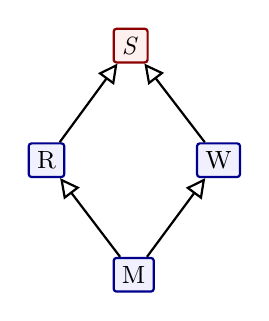
\begin{tikzpicture}[node distance=8mm]
  % class diagram diamond
  \node[abscls] (S) {\textit{S}};
  \node[cls] (R) [below left=10mm and 6mm of S] {R};
  \node[cls] (W) [below right=10mm and 6mm of S] {W};
  \node[cls] (M) [below right=10mm and 6mm of R] {M};
  \draw[isa] (R) -- (S);
  \draw[isa] (W) -- (S);
  \draw[isa] (M) -- (R);
  \draw[isa] (M) -- (W);
\end{tikzpicture}

\medskip
\begin{minipage}[t]{0.46\linewidth}\centering
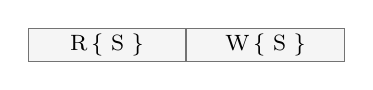
\begin{tikzpicture}[font=\footnotesize,node distance=0pt]
  \node[mem,minimum width=2.0cm] (a1) {R\,\{ S \}};
  \node[mem,minimum width=2.0cm,right=0pt of a1] (a2) {W\,\{ S \}};
\end{tikzpicture}\\[2pt]
{\small (a) nevirtuální: objekt \texttt{M} obsahuje \textbf{dvě} kopie \texttt{S}}
\end{minipage}\hfill
\begin{minipage}[t]{0.50\linewidth}\centering
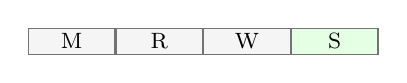
\begin{tikzpicture}[font=\footnotesize,node distance=0pt]
  \node[mem,minimum width=1.1cm] (b1) {M};
  \node[mem,minimum width=1.1cm,right=0pt of b1] (b2) {R};
  \node[mem,minimum width=1.1cm,right=0pt of b2] (b3) {W};
  \node[mem,minimum width=1.1cm,right=0pt of b3,fill=green!10] (b4) {S};
\end{tikzpicture}\\[2pt]
{\small (b) virtuální: jen \textbf{jedna} sdílená \texttt{S}}
\end{minipage}
\end{center}
\obrpopis{Diamantová hierarchie \texttt{M : R, W} a \texttt{R, W : S}. Bez virtuální dědičnosti (a) má objekt \texttt{M} dvě nezávislé kopie \texttt{S} (přístup \texttt{m.S::x} je nejednoznačný). S virtuální dědičností (b) všechny cesty sdílejí jedinou \texttt{S} uloženou na konci rozložení objektu.}

\begin{csalt}[bez vícenásobné dědičnosti]
C\# vícenásobnou dědičnost \emph{tříd} nemá: každá třída má nejvýš \textbf{jednu} bázovou třídu. Celý diamantový problém (dvě kopie báze, virtuální dědičnost, dopočítávané offsety) v~něm proto \textbf{nevzniká} a nemusíte ho vysvětlovat. „Více předků`` se modeluje jako jedna bázová třída plus libovolný počet \emph{rozhraní} (viz výše): \lstinline[style=cs]!class M : Base, I1, I2!. Rozhraní nenesou instanční data, takže se stav nemá jak zdvojit.

\emph{Pozn.:} od C\# 8 mohou mít rozhraní \emph{výchozí implementaci} metod (DIM); i tak ale nenesou žádný instanční stav (duplicita stavu nehrozí) a případnou kolizi dvou stejně pojmenovaných metod řeší \emph{explicitní} implementace.
\end{csalt}

\subsection{Vhodné použití: dědičnost vs. kompozice}

\begin{intuice}
Dědičnost v C++ je silný, ale často zneužívaný nástroj. Bednárek uvádí jen dvě „správná`` použití: (1) \textbf{IS-A hierarchie} entit s vlastní identitou (jednoduchá nevirtuální veřejná dědičnost) a (2) \textbf{vztah rozhraní--implementace} (potomek implementuje abstraktní rozhraní; typicky vícenásobná virtuální veřejná dědičnost, rozhraní bez datových položek). Pro \emph{sdílení/znovupoužití kódu} dědičnost \emph{není} správný nástroj -- na to se hodí \textbf{kompozice} (mít cizí objekt jako datovou položku).
\end{intuice}

\begin{poznamka}[Dva světy tříd]
Kurz odlišuje \emph{hodnotové typy} (bez dědičnosti a virtuálních metod -- chovají se jako čísla, kopírují a přesouvají se (pravidlo pěti, sekce~5), ukládají se přímo, mají smysluplné operátory; např. \texttt{std::string}, matice) od \emph{entitních typů s identitou} (dědičnost, virtuální metody, individuální dynamická alokace, drží se přes ukazatele na společnou bázi, nutný virtuální destruktor). Polymorfní kontejner je vždy \cd{std::vector<std::unique_ptr<Base>>}, nikdy \cd{std::vector<Base>} (slicing).
\end{poznamka}

\begin{priklad}[SZZ jaro 2023 č.~2: Objektový návrh bitmapového editoru]
\szzotazka{jaro 2023}{2}{Objektový návrh (bitmapový editor, polymorfismus, pluginy/DLL)}\par

\textbf{Zadání.}\par
Přepracujte objektový návrh aplikace pro úpravu bitmapových obrázků. Aplikace umí mít otevřeno více obrázků; formát se pozná podle přípony souboru; na obrázek se postupně vybírají filtry, které se nakonec dávkově aplikují; obrázek lze uložit ve stejném či jiném formátu. \emph{Nové filtry} se budou doplňovat přímo do kódu aplikace, kdežto \emph{nové formáty} se budou přidávat jako \emph{pluginy} (dynamicky linkované knihovny) načítané za běhu -- proces načítání obrázku tedy musí být dostatečně flexibilní, aby uměl za běhu přijmout odkaz na nový formát. Navrhněte typy a jejich vztahy v syntaxi zvoleného jazyka a upravte \texttt{Main}. (Původní kostra je v C\#; my odpovídáme v C++.)

\medskip
\textbf{Řešení.}\par
Původní návrh měl chyby: \texttt{Image} mísil \emph{data obrázku} s \emph{načítáním/ukládáním formátu}, filtry byly statické funkce (nešlo je dávkovat ani snadno přidávat) a volba formátu byla natvrdo zadrátovaná v \texttt{ImageLoader} (nešel přidat plugin). Oddělíme proto tři odpovědnosti:

\begin{enumerate}
  \item \textbf{Data obrázku} jako hodnotový typ \texttt{Bitmap} (rozměry + pixely; rozměry filtr nemění).
  \item \textbf{Formát} jako \emph{rozhraní} \texttt{IImageFormat} (\texttt{Load}/\texttt{Save}); každý formát (PNG, JPEG, plugin) je jeho implementace. Registr formátů (\emph{Factory} podle přípony) lze za běhu rozšířit -- sem se zaregistruje plugin.
  \item \textbf{Filtr} jako rozhraní \texttt{IFilter} (\texttt{Apply}); konkrétní filtry nesou svá nastavení. \texttt{Document} drží seznam vybraných filtrů a umí je dávkově aplikovat.
\end{enumerate}

\begin{lstlisting}[style=cpp]
struct Color { uint8_t r, g, b; };

class Bitmap {                       // hodnotový typ: jen data obrázku
    int w_, h_;
    std::vector<Color> px_;          // w_*h_ pixelů
public:
    int width() const { return w_; }
    int height() const { return h_; }
    Color& at(int x, int y) { return px_[y * w_ + x]; }
};

class IImageFormat {                 // rozhraní formátu (implementuje i plugin)
public:
    virtual ~IImageFormat() = default;
    virtual Bitmap Load(const std::string& file) = 0;
    virtual void   Save(const std::string& file, const Bitmap&) = 0;
};
class PngFormat : public IImageFormat { /* Load/Save pro PNG */ };
class JpegFormat : public IImageFormat { /* Load/Save pro JPEG */ };

// Registr formátů = Factory podle přípony; pluginy se sem zaregistrují za běhu.
class FormatRegistry {
    std::map<std::string, std::function<std::unique_ptr<IImageFormat>()>> reg_;
public:
    void Register(const std::string& ext,
                  std::function<std::unique_ptr<IImageFormat>()> factory) {
        reg_[ext] = std::move(factory);
    }
    std::unique_ptr<IImageFormat> Create(const std::string& ext) const {
        auto it = reg_.find(ext);
        if (it == reg_.end()) throw std::runtime_error("neznámý formát");
        return it->second();         // vyrobí instanci formátu
    }
};

class IFilter {                      // rozhraní filtru
public:
    virtual ~IFilter() = default;
    virtual void Apply(Bitmap&) = 0;
};
class Sharpness : public IFilter {
    float amount_, radius_;
public:
    Sharpness(float a, float r) : amount_(a), radius_(r) {}
    void Apply(Bitmap&) override { /* ... */ }
};
class Brightness : public IFilter {
    float amount_;
public:
    explicit Brightness(float a) : amount_(a) {}
    void Apply(Bitmap&) override { /* ... */ }
};

class Document {                     // jeden otevřený obrázek
    Bitmap data_;
    std::unique_ptr<IImageFormat> format_;        // jak se ukládá
    std::vector<std::unique_ptr<IFilter>> filters_;
public:
    void AddFilter(std::unique_ptr<IFilter> f) { filters_.push_back(std::move(f)); }
    void ApplyAll() { for (auto& f : filters_) f->Apply(data_); filters_.clear(); }
    void Save(const std::string& file) { format_->Save(file, data_); }   // v původním formátu
    // uložení v JINÉM formátu: formát se vybere podle cílové přípony (symetricky k Open)
    void SaveAs(const FormatRegistry& reg, const std::string& file) {
        reg.Create(file.substr(file.rfind('.')))->Save(file, data_);
    }
    // tovární metoda: od jména souboru k načtenému obrázku
    static Document Open(const FormatRegistry& reg, const std::string& file) {
        std::string ext = file.substr(file.rfind('.'));   // přípona
        auto fmt = reg.Create(ext);                        // vybere formát
        Document d;
        d.data_   = fmt->Load(file);
        d.format_ = std::move(fmt);
        return d;
    }
};

int main() {
    FormatRegistry reg;
    reg.Register(".png", [] { return std::make_unique<PngFormat>(); });
    reg.Register(".jpg", [] { return std::make_unique<JpegFormat>(); });
    // (plugin by za běhu zavolal reg.Register pro svůj nový formát)
    Document doc = Document::Open(reg, "a.jpg");
    doc.AddFilter(std::make_unique<Sharpness>(9.0f, 1.3f));
    doc.AddFilter(std::make_unique<Brightness>(1.7f));
    doc.ApplyAll();
    doc.Save("a.jpg");          // v původním formátu
    doc.SaveAs(reg, "b.png");   // nebo v jiném podporovaném formátu (PNG)
}
\end{lstlisting}

\textbf{Proč je návrh dobrý.} Nový filtr = nová třída implementující \texttt{IFilter} (přidá se do kódu, nic dalšího se nemění). Nový formát = nová třída implementující \texttt{IImageFormat} \emph{plus} jeden řádek \texttt{reg.Register} -- a ten řádek může zavolat plugin za běhu, takže registr je flexibilní právě v požadovaném místě. Uložení v \emph{jiném} formátu obstará \texttt{SaveAs}, jež vybere formát podle cílové přípony přes týž registr (\texttt{Save} ukládá v~původním). \texttt{Bitmap} je hodnotový typ, \texttt{IFilter}/\texttt{IImageFormat} jsou entitní (drženy přes \cd{unique_ptr}); RAII (sekce~4) zajistí korektní úklid.

\begin{center}
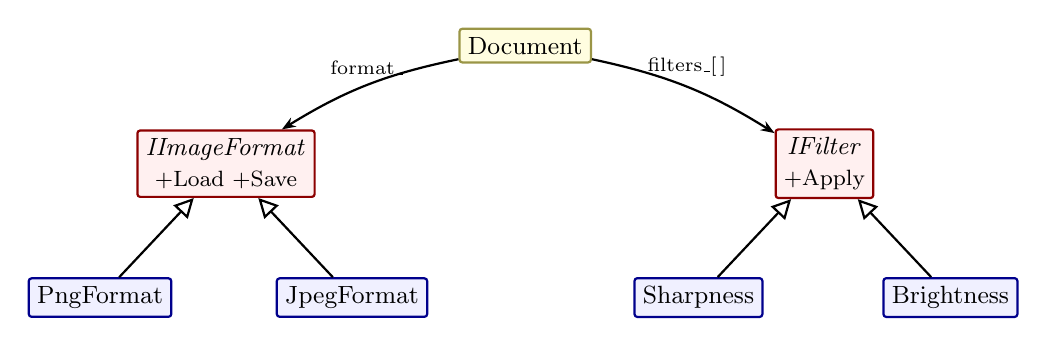
\begin{tikzpicture}[font=\small]
  % levý strom: IImageFormat
  \node[abscls] (ifmt) at (0,0) {\textit{IImageFormat}\\\footnotesize+Load +Save};
  \node[cls] (png) at (-1.6,-1.7) {PngFormat};
  \node[cls] (jpg) at ( 1.6,-1.7) {JpegFormat};
  \draw[isa] (png) -- (ifmt);
  \draw[isa] (jpg) -- (ifmt);
  % pravý strom: IFilter (dostatečně daleko, ať nekoliduje s JpegFormat)
  \node[abscls] (ifil) at (7.6,0) {\textit{IFilter}\\\footnotesize+Apply};
  \node[cls] (sh) at (6.0,-1.7) {Sharpness};
  \node[cls] (br) at (9.2,-1.7) {Brightness};
  \draw[isa] (sh) -- (ifil);
  \draw[isa] (br) -- (ifil);
  % Document drží oba: format_ a filters_[]
  \node[cls,fill=yellow!12,draw=yellow!55!black] (doc) at (3.8,1.5) {Document};
  \draw[ptr] (doc) to[bend right=10] node[midway,above,font=\scriptsize] {format\_} (ifmt);
  \draw[ptr] (doc) to[bend left=10] node[midway,above,font=\scriptsize] {filters\_[\,]} (ifil);
\end{tikzpicture}
\obrpopis{Přepracovaný návrh: \texttt{Document} drží jeden \texttt{IImageFormat} (jak ukládat) a seznam \texttt{IFilter} (co aplikovat). Obě jsou abstraktní rozhraní (červeně), konkrétní formáty i filtry z nich dědí (modře). Přidání filtru = nová třída pod \texttt{IFilter}; přidání formátu = nová třída pod \texttt{IImageFormat} plus registrace v \texttt{FormatRegistry}.}
\end{center}
\end{priklad}

\begin{priklad}[SZZ jaro 2025 č.~2: Knihovna pro výpočty s maticemi]
\szzotazka{jaro 2025}{2}{Knihovna pro výpočty s maticemi (kontrakt/rozhraní)}\par

\textbf{Zadání.}\par
\begin{enumerate}
  \item Definujte \emph{kontrakt} (bez implementace) pro 2D matici: získání rozměrů, hodnoty na souřadnicích, aritmetické operace.
  \item Vytvořte implementaci vhodnou pro velmi velké \emph{řídké} (sparse) matice; implementujte jen rozměry a získání hodnoty a uveďte prostorovou složitost $O(\cdot)$.
  \item S využitím vhodného návrhového vzoru implementujte prostředek, který dostane soubor a vrátí instanci kontraktu s ideální implementací.
\end{enumerate}

\medskip
\textbf{Řešení.}\par
\textbf{(1) Kontrakt} = abstraktní třída (rozhraní) s čistě virtuálními metodami; aritmetiku necháme vracet novou matici přes \cd{unique_ptr<Matrix>} (polymorfní výsledek):

\begin{lstlisting}[style=cpp]
class Matrix {
public:
    virtual ~Matrix() = default;
    virtual int rows() const = 0;
    virtual int cols() const = 0;
    virtual double at(int r, int c) const = 0;          // hodnota na souřadnicích
    virtual std::unique_ptr<Matrix> add(const Matrix&) const = 0;
    virtual std::unique_ptr<Matrix> mul(const Matrix&) const = 0;
};
\end{lstlisting}

\textbf{(2) Řídká implementace -- formát CSR} (Compressed Sparse Row): tři pole -- \texttt{vals\_} (nenulové hodnoty po řádcích), \texttt{cols\_} (jejich sloupce) a \texttt{rowPtr\_} (index, kde v polích začíná každý řádek). Uloží se jen $\mathit{nnz}$ nenulových hodnot, ne $r\cdot c$ nul. \texttt{at} prohledá příslušný úsek řádku:

\begin{lstlisting}[style=cpp]
class SparseMatrix : public Matrix {
    int r_, c_;
    std::vector<double> vals_;       // nenulové hodnoty, seřazené po řádcích
    std::vector<int>    cols_;       // sloupcový index každé hodnoty
    std::vector<int>    rowPtr_;     // rowPtr_[i].. rowPtr_[i+1] = úsek řádku i
public:
    int rows() const override { return r_; }
    int cols() const override { return c_; }
    double at(int r, int c) const override {
        for (int k = rowPtr_[r]; k < rowPtr_[r + 1]; ++k)   // jen nenuly v řádku r
            if (cols_[k] == c) return vals_[k];
        return 0.0;                                          // jinak je tam nula
    }
    std::unique_ptr<Matrix> add(const Matrix&) const override { /* ... */ return {}; }
    std::unique_ptr<Matrix> mul(const Matrix&) const override { /* ... */ return {}; }
};
\end{lstlisting}

Paměť drží jen nenulové prvky a ukazatele na řádky, takže \textbf{prostorová složitost je} $\boxed{O(\mathit{nnz} + r)}$, kde $\mathit{nnz}$ je počet nenulových hodnot a $r$ počet řádků (pole \texttt{rowPtr\_} má délku $r+1$). To je proti hustému $O(r\cdot c)$ obrovská úspora, je-li většina prvků nula.

\textbf{(3) Factory podle obsahu souboru.} Prostředek načte soubor, odhadne hustotu a vrátí ideální implementaci za rozhraním \texttt{Matrix} (tovární metoda vracející \cd{unique_ptr<Matrix>}; konstruktory \texttt{SparseMatrix}/\texttt{DenseMatrix} z~cesty k~souboru zde nevypisujeme):

\begin{lstlisting}[style=cpp]
std::unique_ptr<Matrix> createMatrix(const std::string& path) {
    double density = estimateDensity(path);     // podíl nenulových prvků
    if (density < 0.1) return std::make_unique<SparseMatrix>(path);
    else               return std::make_unique<DenseMatrix>(path);
}
\end{lstlisting}

Volající pracuje jen s rozhraním \texttt{Matrix}, konkrétní implementace je skrytá -- to je smysl návrhového vzoru \emph{Factory}.

\begin{poznamka}
Náčrt v PDF zmiňuje i variantu s \emph{přetíženými operátory} (\cd{operator+}, \cd{operator*}) místo metod \texttt{add}/\texttt{mul} -- v C++ idiomatické pro hodnotové matice. U polymorfního kontraktu drženého přes ukazatel je ale obvyklejší pojmenovaná virtuální metoda; operátory by se daly přidat jako nevirtuální obal volající \texttt{add}/\texttt{mul}.
\end{poznamka}
\end{priklad}

% ============================================================
\section{Primitivní a objektové typy a jejich reprezentace}

C++ má dvě velké skupiny typů: \emph{primitivní} (vestavěné: čísla, znaky, \cd{bool}, výčty, ukazatele) a \emph{složené/objektové} (třídy, struktury, pole, kontejnery). Liší se tím, jak se s nimi zachází a jak vypadají v paměti.

\subsection{Číselné a výčtové typy}

\begin{definice}[Číselné typy]
\emph{Celá čísla}: \cd{int}, \cd{short}, \cd{long}, \cd{long long} a jejich \cd{unsigned} varianty; znaménková se ukládají ve \emph{dvojkovém doplňku}. \emph{Čísla s plovoucí řádovou čárkou}: \cd{float} (32 bitů), \cd{double} (64 bitů), na běžných platformách podle normy IEEE~754 (standard C++ ji nevyžaduje). Velikost typu v bajtech vrací operátor \cd{sizeof}. Pevné velikosti zaručují typy z \texttt{<cstdint>} (\cd{int32_t}, \cd{uint8_t}, \ldots).
\end{definice}

\begin{poznamka}
Přesné bitové reprezentace (dvojkový doplněk, IEEE~754, zarovnání) jsou doménou okruhu \textbf{I4}; zde stačí vědět, že primitivní typy mají \emph{pevnou velikost danou platformou} a ukládají se přímo (žádná dynamická alokace, žádná hlavička objektu).
\end{poznamka}

\begin{definice}[Výčtový typ]
\emph{Výčet} je typ s konečnou množinou pojmenovaných hodnot. Moderní C++ preferuje \emph{silně typovaný} výčet \cd{enum class}:
\end{definice}

\begin{lstlisting}[style=cpp]
enum class Color { Red, Green, Blue };     // silně typovaný (scoped)
Color c = Color::Red;                       // nutná kvalifikace Color::
int i = static_cast<int>(c);                // konverze jen explicitně
enum class Status : uint8_t { Ok, Error };  // lze zvolit podkladový typ
\end{lstlisting}

\begin{intuice}
Starší prostý \cd{enum} se implicitně převádí na \cd{int} a jeho názvy „vytékají`` do okolního jmenného prostoru (riziko kolizí). \cd{enum class} obojí zakazuje: hodnoty jsou v jmenném prostoru výčtu (\texttt{Color::Red}) a konverze na číslo je jen explicitní. Proto je v moderním C++ výchozí volbou.
\end{intuice}

\subsection{Hodnota, ukazatel, reference}

C++ pojmem \emph{odkaz} zastřešuje několik prostředků, jak se dostat k objektu jinde v paměti. Volba odkazu \textbf{signalizuje úmysl} programátora (kdo vlastní, kdo jen čte, jak dlouho).

\begin{definice}[Hodnota, ukazatel, reference]
\begin{itemize}
  \item \emph{Hodnota} (\cd{T x;}) -- proměnná \emph{je} objektem; přístup přes \cd{.}; přiřazení \emph{kopíruje} obsah.
  \item \emph{Ukazatel} (\cd{T* p;}) -- drží \emph{adresu} objektu; přístup přes \cd{*p} a \cd{p->m}; lze ho přesměrovat i nastavit na \cd{nullptr}; umožňuje ukazatelovou aritmetiku v polích.
  \item \emph{Reference} (\cd{T& r = x;}) -- \emph{alias} existujícího objektu; musí být inicializována, \textbf{nelze ji přesměrovat}; přístup přes \cd{.} jako u hodnoty.
\end{itemize}
\end{definice}

\begin{definice}[const reference, r-value reference]
\emph{Konstantní reference} \cd{const T&} váže libovolný výraz (i dočasný) a nedovolí jej měnit -- typický \emph{vstupní parametr} předávaný bez kopie. \emph{R-value reference} \cd{T&&} váže jen \emph{dočasné} (r-value) objekty, „jejichž majitel se o ně už nezajímá``; je základem \emph{move sémantiky} (přesun obsahu místo kopie, viz sekce~5).
\end{definice}

\begin{intuice}
V Javě a C\# se k objektům tříd (tzv.\ referenčním typům) přistupuje vždy přes referenci; C++ naopak u každého typu dává na výběr mezi hodnotou, ukazatelem a referencí. \cd{const T&} jako parametr znamená „jen se podívám, nezdržuj kopírováním``; \cd{T&} „budu měnit tvůj objekt``; \cd{T*} „možná žádný objekt není (\texttt{nullptr})``; \cd{T&&} „tenhle dočasný objekt si rozeberu``.
\end{intuice}

\subsection{Vlastník vs. pozorovatel, zásobník vs. halda}

Klíčový myšlenkový model kurzu: každý odkaz je buď \emph{vlastník} (owner), který je zodpovědný za zrušení objektu, nebo \emph{pozorovatel} (observer), který objekt jen používá a nesmí ho rušit.

\begin{definice}[Vlastník a pozorovatel]
\emph{Vlastník} drží objekt a uvolní ho, až přestane být potřeba: \cd{std::unique_ptr<T>} (výhradní vlastník), \cd{std::shared_ptr<T>} (sdílený vlastník). \emph{Pozorovatel} jen odkazuje, nevlastní: holý \cd{T*} (měnící), \cd{const T*} (jen čtoucí) nebo reference. V moderním C++ \textbf{holý ukazatel nikdy nereprezentuje vlastnictví}.
\end{definice}

\begin{poznamka}[Kde objekt žije]
\emph{Statická} doba života: globální a \cd{static} proměnné (žijí po celý běh). \emph{Automatická} (zásobník): lokální proměnné, rušené automaticky na konci bloku -- rychlé, ale životnost vázaná na blok. \emph{Dynamická} (halda): objekty vytvořené \cd{new} / \cd{make_unique} / \cd{make_shared}, žijí, dokud je někdo neuvolní; pomalejší (cache), nutné jen tam, kde životnost nesouvisí s voláním funkcí nebo kde je objekt polymorfní.
\end{poznamka}

\begin{center}
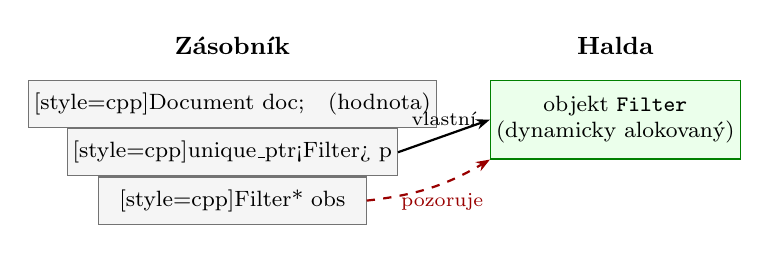
\begin{tikzpicture}[font=\footnotesize,node distance=0pt]
  % stack
  \node[font=\small\bfseries] (st) {Zásobník};
  \node[mem,minimum width=3.4cm,minimum height=6mm,below=2mm of st.south,anchor=north] (s1) {\cd{Document doc;}\quad(hodnota)};
  \node[mem,minimum width=3.4cm,minimum height=6mm,below=0pt of s1] (s2) {\cd{unique_ptr<Filter> p}};
  \node[mem,minimum width=3.4cm,minimum height=6mm,below=0pt of s2] (s3) {\cd{Filter* obs}};
  % heap
  \node[font=\small\bfseries,right=34mm of st] (hp) {Halda};
  \node[heapblk,minimum width=3.0cm,minimum height=10mm,below=2mm of hp.south,anchor=north] (h1) {objekt \texttt{Filter}\\(dynamicky alokovaný)};
  % arrows
  \draw[ptr] (s2.east) -- node[above,font=\scriptsize]{vlastní} (h1.west);
  \draw[ptr,dashed,red!60!black] (s3.east) to[bend right=12] node[below,font=\scriptsize,pos=0.6]{pozoruje} (h1.south west);
\end{tikzpicture}
\obrpopis{Zásobník drží malé „úchyty`` s automatickou dobou života; samotné objekty leží na haldě. \cd{unique_ptr} \texttt{p} haldový objekt \emph{vlastní} (zruší ho ve svém destruktoru, plná šipka). Holý ukazatel \texttt{obs} týž objekt jen \emph{pozoruje} (přerušovaná šipka) -- nevlastní ho a nesmí ho rušit; musí přestat pozorovat dřív, než vlastník objekt zruší. Hodnotový objekt \texttt{doc} žije přímo na zásobníku.}
\end{center}

% ============================================================
\section{Generické typy, funkcionální prvky, lambda funkce}

Generické programování umožňuje napsat kód jednou a použít ho pro mnoho typů. C++ k tomu má \emph{šablony} (templates), které pracují \emph{za překladu} -- to je základ \emph{statického polymorfismu}. Funkcionální prvky (ukazatele na funkce, funktory, lambdy, \cd{std::function}) umožňují předávat „chování`` jako hodnotu.

\subsection{Šablony (generické typy)}

\begin{definice}[Šablona]
\emph{Šablona} je generická deklarace s \emph{formálními parametry vyhodnocenými za překladu}. Parametrem může být \emph{typ} (\cd{template<typename T>}), \emph{celočíselná konstanta} (\cd{template<std::size_t N>}) nebo jiná šablona. Rozlišujeme \emph{šablonu funkce} a \emph{šablonu třídy}:
\end{definice}

\begin{lstlisting}[style=cpp]
template <typename T>                 // šablona funkce
T max(T a, T b) { return a < b ? b : a; }

template <typename T, std::size_t N>  // šablona třídy
class array { T data_[N]; /* ... */ };

int m = max(3, 7);            // instanciace: T = int (odvozeno z argumentů)
double d = max<double>(1, 2); // T zadáno explicitně
array<int, 10> a;             // instanciace třídy: T = int, N = 10
\end{lstlisting}

\begin{definice}[Instanciace, specializace]
\emph{Instanciace} = použití šablony s konkrétními parametry; teprve tehdy překladač vygeneruje kód. U funkcí se typ často \emph{odvodí} z argumentů, u tříd se zadává explicitně (od C++17 i u tříd lze odvodit, CTAD). \emph{Specializace} dává pro konkrétní parametry jinou definici (úplná \cd{template<> struct hash<MyType>}, nebo částečná -- ta jen u šablon tříd, ne u funkcí, např.\ \cd{template<class A> class vector<bool, A>}).
\end{definice}

\begin{poznamka}
Definice šablony musí být \textbf{viditelná v místě instanciace}, proto šablony bývají celé v hlavičkových souborech (nelze je oddělit do \texttt{.cpp} jako běžné funkce). Šablony nemají \emph{žádnou běhovou režii} -- vygenerovaný kód je stejný, jako by byl napsán ručně pro daný typ; cenou je možné nafouknutí velikosti kódu (každá instanciace je samostatná).
\end{poznamka}

\subsection{Statický vs. dynamický polymorfismus}

\emph{Polymorfismus} je schopnost přizpůsobit chování kódu. C++ ho má ve dvou podobách, které je dobré umět porovnat:

\begin{center}
\renewcommand{\arraystretch}{1.25}
\begin{tabular}{@{}p{0.31\linewidth}p{0.31\linewidth}p{0.31\linewidth}@{}}
\toprule
 & \textbf{Statický (šablony)} & \textbf{Dynamický (virtuální)} \\
\midrule
Kdy se rozhodne & při překladu (instanciace) & za běhu (vtable) \\
Společná báze & netřeba (\emph{duck typing}) & nutná abstraktní třída \\
Signatura & libovolná kompatibilní & přesně daná bází \\
Volání & přímé, lze \emph{inlinovat} & nepřímé přes ukazatel \\
Rychlost & rychlejší & pomalejší \\
Velikost kódu & větší (více instanciací) & menší (jeden kód) \\
Přepínání za běhu & ne & ano \\
\bottomrule
\end{tabular}
\end{center}

\begin{intuice}
\emph{Duck typing} (řádek „společná báze`` v tabulce): šabloně stačí, že typ má použité operace (metody/operátory správného jména a typu), nemusí dědit ze společné báze -- „když to kváká jako kachna, ber to jako kachnu``. Statický polymorfismus je tím volnější než dynamický, který společnou abstraktní bázi vyžaduje. Doporučení kurzu: \textbf{preferuj statický polymorfismus, dynamický jen když je nutný} -- tedy když se chování musí volit až za běhu (polymorfní kontejnery různých typů, GUI prvky, zásuvné moduly). Statický je „zadarmo`` (inlinuje se), ale neumí za běhu přepínat; dynamický to umí, ale platí nepřímým voláním přes tabulku virtuálních metod (sekce~7).
\end{intuice}

\subsection{Typy reprezentující funkce, lambda, funkcionální rozhraní}

Často chceme předat \emph{chování} (porovnávací funkci, operaci na prvku) jako argument. C++ k tomu má tři prostředky:

\begin{definice}[Ukazatel na funkci, funktor, \texttt{std::function}]
\begin{itemize}
  \item \emph{Ukazatel na funkci} \cd{void(*)(int)} -- nejstarší, beze stavu, pevná signatura.
  \item \emph{Funktor} (funkční objekt) -- třída s přetíženým \cd{operator()}; může nést \emph{stav} v datových položkách (uzávěr: tělo + nabalená data).
  \item \cd{std::function<void(int)>} -- typové úložiště pro libovolné volatelné s danou signaturou; dražší (případná dynamická alokace, nepřímé volání), použít, až když je potřeba míchat/ukládat různá volatelná.
\end{itemize}
\end{definice}

\begin{definice}[Lambda funkce]
\emph{Lambda} je výraz \lstinline[style=cpp]![capture](params){ telo }!, který překladač přeloží na \emph{anonymní funktor}. Seznam \emph{capture} určuje, které okolní proměnné lambda zachytí a jak: \cd{[x]} hodnotou (kopie), \cd{[&x]} odkazem, \cd{[=]}/\cd{[&]} vše \emph{použité} hodnotou/odkazem, \cd{[this]} přístup k objektu.
\end{definice}

\begin{lstlisting}[style=cpp]
std::vector<int> v = {3, 1, 2};
int prah = 2;
// lambda zachytí proměnnou prah hodnotou; std::count_if čeká volatelné:
auto kolik = std::count_if(v.begin(), v.end(),
                           [prah](int x){ return x > prah; });
// lambda = anonymní funktor; uloží se do proměnné typu, který zná jen překladač:
auto add = [](int a, int b){ return a + b; };
// pro uložení/míchání různých lambd se stejnou signaturou slouží std::function:
std::function<int(int,int)> op = add;
\end{lstlisting}

\begin{intuice}
Každá lambda má \emph{vlastní anonymní typ}, takže dvě lambdy téže signatury nelze přímo zaměnit ani uložit do jedné proměnné -- na to je právě \cd{std::function}. Funkce přijímající lambdu proto bývají \emph{šablony} (\cd{template<typename F> void g(F f)}): chování se předá v \emph{typu}, vyřeší se za překladu a inlinuje (statický polymorfismus). \emph{Funkcionálním rozhraním} se v C++ míní právě „cokoli volatelné s danou signaturou`` -- ukazatel, funktor, lambda i \cd{std::function}.
\end{intuice}

\begin{priklad}[SZZ podzim 2022 č.~1: Objektové rozhraní pro grafy]
\szzotazka{podzim 2022}{1}{Programování (rozhraní pro grafy)}\par

\textbf{Zadání.}\par
Navrhněte (jen deklarujte) generické objektové rozhraní pro neorientované grafy
$G = (V, E)$ (hrany spojují právě dva vrcholy, mezi dvěma vrcholy nejvýš jedna
hrana), aby je mohly implementovat různé reprezentace (seznam sousedů, matice
sousednosti, \dots) a algoritmy se psaly jen jednou. Rozhraní pokrývá 3~entity:
\emph{vrchol} (přístup k~incidentním hranám), \emph{hrana} (její dva vrcholy)
a~\emph{graf} (seznam všech vrcholů a~hran, pouze pro čtení). Každý vrchol i~hrana
nese \emph{tag} (např. příznak navštívení u~vrcholu, váha u~hrany); typy tagů volí
uživatel, ale v~rámci jedné instance mají všechny vrcholy stejný typ tagu a~všechny
hrany taktéž (rozhraní je tedy generické). Dále napište tělo funkce, která pro daný
graf a~reálné číslo $r$ rozloží graf na komponenty souvislosti, přičemž hrany
s~tagem (délkou) větším než $r$ ignoruje, a~index komponenty každého vrcholu uloží
do jeho tagu.

\medskip
\textbf{Řešení.}\par
\textbf{(1) Tři generická rozhraní.} Parametry \texttt{VTag}/\texttt{ETag} nesou typy
tagů; v~C++ jsou to abstraktní třídy-šablony (čistě virtuální metody), takže algoritmus
je nezávislý na vnitřní reprezentaci grafu:

\begin{lstlisting}[style=cpp]
template <class VTag, class ETag> struct IEdge;        // dopředná deklarace

template <class VTag, class ETag>
struct IVertex {                                       // vrchol
    virtual ~IVertex() = default;
    virtual std::vector<IEdge<VTag,ETag>*> incidentEdges() = 0;  // incidentni hrany
    virtual VTag getTag() const = 0;
    virtual void setTag(VTag) = 0;
};
template <class VTag, class ETag>
struct IEdge {                                         // hrana
    virtual ~IEdge() = default;
    virtual IVertex<VTag,ETag>* endpoint1() = 0;       // jeden koncovy vrchol
    virtual IVertex<VTag,ETag>* endpoint2() = 0;       // druhy koncovy vrchol
    virtual ETag getTag() const = 0;
    virtual void setTag(ETag) = 0;
};
template <class VTag, class ETag>
struct IGraph {                                        // graf je pouze pro cteni
    virtual ~IGraph() = default;
    virtual std::vector<IVertex<VTag,ETag>*> vertices() = 0;
    virtual std::vector<IEdge<VTag,ETag>*>   edges() = 0;
};
\end{lstlisting}

\textbf{(2) Komponenty souvislosti.} BFS z~každého dosud neoznačeného vrcholu;
šíříme se jen po hranách s~tagem $\le r$, ostatní (delší) ignorujeme. Vrcholům
dosaženým v~jednom průchodu nastavíme stejný index, čítač pak zvýšíme. Tagy vrcholů
jsou \cd{int} (index komponenty, $-1$ = neoznačeno), tagy hran \cd{float} (délka):

\begin{lstlisting}[style=cpp]
void connectedComponents(IGraph<int,float>& g, float r) {
    for (auto* v : g.vertices()) v->setTag(-1);        // -1 = neoznaceno
    int component = 0;
    for (auto* start : g.vertices()) {
        if (start->getTag() != -1) continue;           // jiz prirazen
        std::queue<IVertex<int,float>*> q;             // BFS z vrcholu start
        start->setTag(component); q.push(start);
        while (!q.empty()) {
            auto* u = q.front(); q.pop();
            for (auto* e : u->incidentEdges()) {
                if (e->getTag() > r) continue;          // prilis dlouha hrana, ignoruj
                auto* w = (e->endpoint1() == u) ? e->endpoint2() : e->endpoint1();
                if (w->getTag() == -1) { w->setTag(component); q.push(w); }
            }
        }
        component++;                                    // dalsi komponenta
    }
}
\end{lstlisting}

\textbf{Proč to funguje.} Hrany s~tagem $> r$ se v~BFS přeskočí, takže rozklad
odpovídá podgrafu jen s~hranami délky $\le r$. Protože pracujeme výhradně přes
rozhraní (\cd{vertices()}, \cd{incidentEdges()}, \cd{getTag}/\cd{setTag}), je tělo
funkce totožné pro každou reprezentaci grafu -- to je smysl generického rozhraní.
\end{priklad}

\begin{priklad}[SZZ léto 2023 č.~18: Komponentový systém]
\szzotazka{léto 2023}{18}{Komponentový systém (herní framework, generika, komponenty)}\par

\noindent\textit{(Pozn.: v~rámci současné akreditace nešlo o~společnou otázku (q1--q4), ale o~otázku jiné specializace (specializační sekce, ne UI). Do společného okruhu I3 tedy formálně nepatří; tematicky sem ovšem spadá a~je výborná k~procvičení.)}\par

\textbf{Zadání.}\par
Navrhněte komponentový herní framework. Každý objekt scény je \texttt{GameObject} (GO), což je množina \emph{komponent}. Od každého \emph{druhu} komponenty má GO nejvýš jednu instanci. Potřeba je: (1) metoda pro připojení komponenty (stejný druh nahradí předchozí) a pro získání komponenty zvoleného druhu (s indikací, že chybí); metoda \texttt{Update(timeDelta)} zavolá \texttt{Update} na těch komponentách, které ji mají (autor komponenty se rozhodne, zda ji má). (2) Komponenty \texttt{Position} a \texttt{Health}. (3) Efekty otravy a krvácení (vyžadují \texttt{Health}), parametrizované úbytkem zdraví za sekundu; funkce, která zvolený efekt aplikuje na seznam GO.

\medskip
\textbf{Řešení.}\par
\textbf{(1) Identifikace druhu komponenty.} Druh komponenty reprezentujeme jejím \emph{typem} a klíčujeme podle \cd{std::type_index} (běhový identifikátor typu). \texttt{GameObject} drží mapu z typu na komponentu. Generická metoda \cd{Get<T>} vrátí ukazatel na komponentu typu \texttt{T}, nebo \cd{nullptr}, když chybí -- to je ono „rozumné indikování``. Možnost mít/nemít \texttt{Update} řešíme volitelným rozhraním \texttt{IUpdatable}.

\begin{lstlisting}[style=cpp]
struct Component { virtual ~Component() = default; };  // báze všech komponent
struct IUpdatable {                                     // volitelné rozhraní
    virtual ~IUpdatable() = default;
    virtual void Update(float dt) = 0;
};

class GameObject {
    std::unordered_map<std::type_index, std::unique_ptr<Component>> comps_;
public:
    template <typename T>                       // připojení (nahradí stejný druh)
    void Add(std::unique_ptr<T> c) { comps_[std::type_index(typeid(T))] = std::move(c); }

    template <typename T>                       // získání, nebo nullptr když chybí
    T* Get() {
        auto it = comps_.find(std::type_index(typeid(T)));
        return it == comps_.end() ? nullptr : static_cast<T*>(it->second.get());
    }
    void Update(float dt) {                     // zavolá Update na komponentách, co ji mají
        for (auto& [type, c] : comps_)
            if (auto* u = dynamic_cast<IUpdatable*>(c.get())) u->Update(dt);
    }
};
\end{lstlisting}

\textbf{(2) Konkrétní komponenty.}
\begin{lstlisting}[style=cpp]
struct Position : Component { float x = 0, y = 0; };
class Health : public Component {             // invariant: 0 <= cur_ <= max_
    float max_, cur_;
public:
    Health(float max, float cur) : max_(max), cur_(std::clamp(cur, 0.0f, max)) {}
    float Max() const { return max_; }
    float Current() const { return cur_; }
    void SetCurrent(float v) { cur_ = std::clamp(v, 0.0f, max_); }  // hlídá rozsah
};

auto kamen = std::make_unique<GameObject>();
kamen->Add(std::make_unique<Position>());
auto trol = std::make_unique<GameObject>();
trol->Add(std::make_unique<Position>());
trol->Add(std::make_unique<Health>(30.0f, 20.0f));   // max = 30, aktuální = 20
\end{lstlisting}

\textbf{(3) Efekty.} Efekt je komponenta \emph{a zároveň} \texttt{IUpdatable}; v \texttt{Update} si najde \texttt{Health} na svém GO (potřebuje zpětný odkaz na vlastníka) a ubírá zdraví. Otrava i krvácení sdílejí logiku, liší se jen typem: protože \texttt{GameObject} klíčuje komponenty podle typu, musejí to být \emph{dva různé typy} (jinak by druhý efekt přepsal první), aby mohly být na GO obě současně. Volbu „otrava vs. krvácení`` ve funkci řešíme \emph{šablonovým} parametrem typu efektu:

\begin{lstlisting}[style=cpp]
class Effect : public Component, public IUpdatable {
protected:
    GameObject* owner_;  float perSec_;       // pozorovatel vlastníka + parametr
public:
    Effect(GameObject* o, float p) : owner_(o), perSec_(p) {}
    void Update(float dt) override {
        if (auto* hp = owner_->Get<Health>())  // efekt nic nedělá, chybí-li Health
            hp->SetCurrent(hp->Current() - perSec_ * dt);
    }
};
struct Poison   : Effect { using Effect::Effect; };  // dva různé typy,
struct Bleeding : Effect { using Effect::Effect; };  // aby šly na GO obě naráz

template <typename E>                          // volba efektu = typový parametr
void applyEffect(const std::vector<GameObject*>& gos, float perSec) {
    for (GameObject* go : gos)
        if (go->Get<Health>())                 // jen na GO s komponentou Health
            go->Add(std::make_unique<E>(go, perSec));
}
// použití: na kámen a trola zkusíme krvácení 1.2/s (kámen nemá Health -> přeskočí se)
applyEffect<Bleeding>({kamen.get(), trol.get()}, 1.2f);
\end{lstlisting}

\textbf{Komentář k volbám.} Klíčování podle typu (\cd{type_index}) splní „nejvýš jedna instance daného druhu`` zdarma; držení přes \cd{unique_ptr} zaručí, že komponenta patří nejvýš jednomu GO. \texttt{Health} je zapouzdřená, takže invariant $0 \le \text{cur} \le \text{max}$ ze zadání hlídá jediné místo (\texttt{SetCurrent}). \cd{Get<T>} vrací \cd{nullptr} při absenci -- vhodná indikace pro dotaz „má GO tuto komponentu?{}``. Volitelnost \texttt{Update} přes \texttt{IUpdatable} + \cd{dynamic_cast} respektuje, že ne každá komponenta \texttt{Update} má. Volbu efektu jsme dali do \emph{šablonového} parametru (statický polymorfismus) -- alternativně by šel běhový příznak nebo tovární funkce.
\end{priklad}

\begin{priklad}[SZZ podzim 2024 č.~2: Reprezentace typů (návrh + Visitor)]
\szzotazka{podzim 2024}{2}{Reprezentace typů (návrh tříd/interfaců pro IDE)}\par

\textbf{Zadání.}\par
(1) Pro IDE navrhněte třídy/rozhraní pro uchování informací o typech a jejich elementech (metody, datové položky, vnořené typy) tak, aby šlo snadno rozšiřovat; jen deklarace. (2) Implementujte metodu, která na typ a všechny jeho elementy aplikuje zadanou „operaci`` -- pokud použijete obecně známé řešení průchodu, pojmenujte ho; pro operaci použijte vhodný koncept jazyka. (3) Zavolejte metodu s operací „vytiskni název elementu, jen jde-li o datovou položku nebo typ``.

\medskip
\textbf{Řešení.}\par
\textbf{(1) Hierarchie elementů.} Společná abstraktní báze \texttt{Element}, z níž dědí \texttt{Type}, \texttt{Method}, \texttt{Field}. Typ obsahuje své elementy (kompozice); vnořené typy jsou opět \texttt{Type}, takže struktura je rekurzivní (strom).

\begin{lstlisting}[style=cpp]
struct Visitor;                              // dopředná deklarace
struct Element {
    virtual ~Element() = default;
    std::string name;
    virtual void accept(Visitor& v) = 0;     // Visitor: double dispatch
};
struct Field  : Element { std::string type; void accept(Visitor&) override; };
struct Method : Element { std::string signature; void accept(Visitor&) override; };
struct Type   : Element {                    // typ drží své elementy (i vnořené typy)
    std::vector<std::unique_ptr<Element>> members;
    void accept(Visitor&) override;
};
\end{lstlisting}

\textbf{(2) Průchod = návrhový vzor \emph{Visitor}.} Operaci pojmeme jako \emph{návštěvníka} s metodou \texttt{visit} pro každý druh elementu; metoda \texttt{accept} na elementu zavolá správnou \texttt{visit} (dvojitá dispatch). Průchod typem aplikuje návštěvníka na typ i rekurzivně na všechny elementy:

\begin{lstlisting}[style=cpp]
struct Visitor {
    virtual void visit(Field&)  = 0;
    virtual void visit(Method&) = 0;
    virtual void visit(Type&)   = 0;
};
void Field::accept(Visitor& v)  { v.visit(*this); }
void Method::accept(Visitor& v) { v.visit(*this); }
void Type::accept(Visitor& v) {
    v.visit(*this);
    for (auto& m : members) m->accept(v);    // rekurzivně na elementy (i vnořené typy)
}
\end{lstlisting}

\textbf{(3) Konkrétní operace.} Operaci „vytiskni název jen u datové položky nebo typu`` realizujeme konkrétním návštěvníkem (a v \texttt{main} ho použijeme). Pro pohodlí by šly metody \texttt{visit} delegovat na uloženou \emph{lambdu}, ale s rozhraním \texttt{Visitor} je nejpřímější odvodit třídu:

\begin{lstlisting}[style=cpp]
struct PrintNamesVisitor : Visitor {
    void visit(Field& f)  override { std::cout << f.name << "\n"; }  // tiskne
    void visit(Type& t)   override { std::cout << t.name << "\n"; }  // tiskne
    void visit(Method&)   override { /* metodu netiskne */ }
};
void run(Type& root) {
    PrintNamesVisitor pv;
    root.accept(pv);                          // projde typ i všechny jeho elementy
}
\end{lstlisting}

\begin{poznamka}
Náčrt v PDF jmenuje právě \emph{Visitor} (případně „sealed`` typy + pattern matching v jazycích, co to mají); operace může být rozhraní, funkcionální typ, anonymní třída či \emph{lambda}. V C++ je idiomatická buď hierarchie \texttt{Visitor} (zde), nebo \cd{std::variant} elementů $+$ \cd{std::visit} s lambdou (pattern matching). Rozšiřitelnost o nový druh elementu při Visitoru znamená přidat metodu \texttt{visit} do rozhraní (a doimplementovat ji ve všech existujících návštěvnících) -- Visitor se proto hodí pro stabilní hierarchie.
\end{poznamka}
\end{priklad}

\begin{csalt}[pattern matching místo Visitoru]
U předchozí otázky náčrt v PDF přímo zmiňuje „sealed typy + pattern matching`` -- a pattern matching je v~C\# běžný idiom. Místo dvojité dispatche (\texttt{accept}/\texttt{visit}) stačí jeden \cd{switch} se vzory typů; nepotřebujete rozhraní \texttt{Visitor} ani metodu \texttt{accept} v~každém typu. (Listové třídy lze označit \cd{sealed}, tím se ale v~C\# jen zakáže další dědění; úplnost \cd{switch} přes celou hierarchii překladač nekontroluje. To umí až Java: uzavřené hierarchie \texttt{sealed \dots{} permits} má od verze~17, \cd{switch} s~typovými vzory a~kontrolou úplnosti od verze~21.)
\begin{lstlisting}[style=cs]
void Visit(Element e) {
    switch (e) {
        case Field f: Console.WriteLine(f.name); break;                  // tiskni
        case Type t:  Console.WriteLine(t.name);
                      foreach (var m in t.members) Visit(m); break;       // rekurze
        case Method:  break;                                             // metodu netiskni
    }
}
\end{lstlisting}
Přidat \emph{operaci} je pak triviální (nová funkce se \cd{switch}). Cenou je opačný kompromis než u Visitoru: přidání nového \emph{druhu} elementu si vynutí úpravu všech \cd{switch} (kdežto u Visitoru se mění rozhraní). Pro typické zadání „aplikuj operaci na strom typů`` je ale C\# verze výrazně kratší.
\end{csalt}

% ============================================================
\section{Manipulace se zdroji a ošetření chyb (výjimky)}

\emph{Zdroj} je něco, co se musí po použití uvolnit: paměť, otevřený soubor, zámek, síťové spojení. V C++ se o uvolnění stará \emph{RAII}, a to spolehlivě i tehdy, když výpočet přeruší \emph{výjimka}. Tato dvě témata spolu úzce souvisí.

\subsection{RAII: vázání zdroje na životnost objektu}

\begin{definice}[RAII]
\emph{RAII} (Resource Acquisition Is Initialization) je idiom, kdy \textbf{získání zdroje} svážeme s \emph{konstrukcí} objektu a \textbf{uvolnění zdroje} s jeho \emph{destrukcí}. Objekt zdroj \emph{vlastní}; jeho destruktor zdroj uvolní automaticky na konci platnosti objektu, ať se z bloku odejde jakkoli (normálně, \cd{return}, nebo výjimkou).
\end{definice}

\begin{intuice}
RAII je v C++ \emph{hlavní} mechanismus správy zdrojů a nahrazuje konstrukci \texttt{try}/\texttt{finally} z jiných jazyků (kterou C++ \textbf{nemá}). Místo „nezapomeň v každé větvi uvolnit`` se zdroj uvolní sám v destruktoru. Příkladem jsou \cd{std::unique_ptr} (vlastní paměť), \cd{std::lock_guard} (vlastní zámek), \cd{std::fstream} (vlastní soubor).
\end{intuice}

\begin{lstlisting}[style=cpp]
void prenes(Ucet& z, Ucet& na, int castka) {
    std::lock_guard<std::mutex> g(z.mtx);  // zamkne v konstruktoru
    z.zustatek -= castka;
    na.zustatek += castka;
}   // ~lock_guard() odemkne mutex i kdyby zde výpočet skončil výjimkou
\end{lstlisting}

\subsection{Výjimky: vyhození, zachycení, propagace}

\begin{definice}[Výjimka, \texttt{throw}/\texttt{try}/\texttt{catch}]
\emph{Výjimka} je objekt vyhozený příkazem \cd{throw} při chybovém stavu. Vyhození ukončí běžný tok a hledá nejbližší obklopující blok \cd{try} s \cd{catch}, jehož typ odpovídá (podle dědičnosti) typu vyhozené hodnoty. Nenajde-li se žádný, zavolá se \cd{std::terminate} a program skončí.
\end{definice}

\begin{definice}[Odvíjení zásobníku (stack unwinding)]
Při hledání odpovídajícího \cd{catch} se postupně opouštějí bloky a funkce na zásobníku; přitom se \textbf{volají destruktory všech lokálních objektů} v opouštěných rámcích. Tomuto procesu se říká \emph{odvíjení zásobníku}. Právě díky němu RAII uvolní zdroje i při výjimce.
\end{definice}

\begin{lstlisting}[style=cpp]
struct ChybaSouboru : std::runtime_error {     // vlastní výjimka dědí z std::
    using std::runtime_error::runtime_error;
};
void f() {                                     // vyhodí výjimku
    throw ChybaSouboru("nelze zapsat");
}
void g() {
    std::ofstream out("a.txt");                // RAII zdroj v g()
    f();                                       // f() vyhodí; pak ~ofstream
}   // při opuštění g() se out korektně zavře (unwinding)
int main() {
    try {
        g();
    } catch (const std::exception& e) {        // chytá i potomky (dědičnost)
        std::cerr << "chyba: " << e.what() << "\n";
    }
}
\end{lstlisting}

\begin{poznamka}
Standardní výjimky dědí z \cd{std::exception} (metoda \cd{what()} vrací popis); dělí se na \cd{std::logic_error} (chyba programátora: \cd{out_of_range}, \cd{invalid_argument}) a \cd{std::runtime_error} (problém za běhu). Vlastní výjimky je dobré odvozovat z \cd{std::exception}. Chytáme \emph{referencí} (\cd{const std::exception&}), aby fungovala dědičnost a nedošlo ke slicingu; \cd{throw;} bez argumentu výjimku \emph{přehodí} dál (rethrow).
\end{poznamka}

\begin{center}
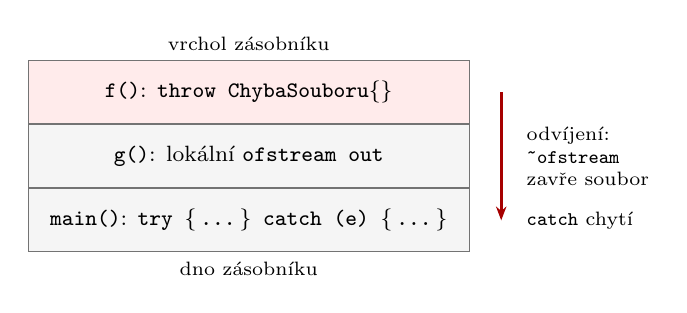
\begin{tikzpicture}[font=\footnotesize,node distance=0pt]
  % stack frames bottom -> top
  \node[mem,minimum width=5.6cm,minimum height=8mm] (main) {\texttt{main()}: \texttt{try \{\,...\,\} catch (e) \{\,...\,\}}};
  \node[mem,minimum width=5.6cm,minimum height=8mm,above=0pt of main] (g)
       {\texttt{g()}: lokální \texttt{ofstream out}};
  \node[mem,minimum width=5.6cm,minimum height=8mm,above=0pt of g,fill=red!8] (f)
       {\texttt{f()}: \texttt{throw ChybaSouboru\{\}}};
  \node[anchor=south,font=\scriptsize] at (f.north) {vrchol zásobníku};
  \node[anchor=north,font=\scriptsize] at (main.south) {dno zásobníku};
  % unwinding: šipka dolů po pravé straně od f k main (směr propagace)
  \draw[ptr,red!65!black,line width=1pt] ([xshift=4mm]f.east) -- ([xshift=4mm]main.east);
  \node[right,font=\scriptsize,align=left] at ([xshift=6mm]g.east)
       {odvíjení:\\ \texttt{\textasciitilde ofstream}\\ zavře soubor};
  \node[right,font=\scriptsize] at ([xshift=6mm]main.east) {\texttt{catch} chytí};
\end{tikzpicture}
\obrpopis{Schematický řetězec volání \texttt{main} $\to$ \texttt{g} $\to$ \texttt{f}. Funkce \cd{f()} vyhodí výjimku; ta se propaguje zpět volajícími rámci (\texttt{g}, pak \texttt{main}) k prvnímu odpovídajícímu \cd{catch} v \cd{main()}. Při opouštění mezilehlého rámce \cd{g()} se zavolá destruktor jeho lokálního \cd{ofstream}, který zavře soubor -- tak RAII zaručí úklid zdrojů i při chybě (C++ nepotřebuje \texttt{finally}).}
\end{center}

\subsection{Bezpečnost vůči výjimkám; proč destruktory nehází}

\begin{definice}[Úrovně záruky bezpečnosti vůči výjimkám]
\begin{itemize}
  \item \emph{Základní} (basic): i při výjimce zůstanou data v \emph{konzistentním} stavu (žádné úniky, platné invarianty).
  \item \emph{Silná} (strong): operace buď proběhne celá, nebo nezmění pozorovatelný stav (\emph{commit-or-rollback}).
  \item \emph{Nothrow} (\cd{noexcept}): operace výjimku nikdy nevyhodí.
\end{itemize}
\end{definice}

\begin{poznamka}
\textbf{Destruktor nesmí vyhodit výjimku} a je implicitně \cd{noexcept}. Důvod: při odvíjení zásobníku už jedna výjimka „letí``; kdyby destruktor vyhodil druhou, nelze obě zpracovat a volá se \cd{std::terminate}. Proto se v destruktorech nedělají operace, které mohou selhat. Související idiom: \emph{move} operace značíme \cd{noexcept}, jinak je kontejnery (např. \cd{std::vector} při realokaci) z bezpečnostních důvodů nevyužijí a raději kopírují.
\end{poznamka}

% ============================================================
\section{Životní cyklus objektů a správa paměti (GC, reference counting)}

Životní cyklus objektu má tři fáze: \emph{alokace} (kde vznikne), \emph{inicializace} (konstruktor) a \emph{destrukce} (destruktor). C++ dává programátorovi kontrolu nad všemi třemi a nemá garbage collector -- paměť se uvolňuje deterministicky (RAII, chytré ukazatele).

\subsection{Alokace a inicializace}

\begin{poznamka}[Tři druhy alokace]
\emph{Statická} (globální/\cd{static}): jediná instance, žije po celý běh. \emph{Na zásobníku} (automatická): lokální proměnné, vznikají a zanikají s blokem, velmi rychlé. \emph{Na haldě} (dynamická): \cd{new}/\cd{make_unique}/\cd{make_shared}, žijí nezávisle na voláních funkcí, dokud je někdo neuvolní.
\end{poznamka}

\begin{poznamka}[Explicitní uvolňování a proč se mu vyhýbáme]
Haldu lze obsluhovat ručně: \cd{T* p = new T;} alokuje, \cd{delete p;} uvolní. Ruční pár je ale křehký -- zapomenutý \cd{delete} je únik paměti, dvojí \cd{delete} nebo \cd{delete} po výjimce je nedefinované chování. Proto moderní C++ alokaci na haldě skoro vždy svěřuje chytrým ukazatelům (\cd{make_unique}/\cd{make_shared}), které uvolní automaticky (RAII, sekce~4) -- explicitní \cd{delete} v~aplikačním kódu je dnes spíš výjimkou. To je protějšek \emph{garbage collectoru} ze spravovaných jazyků (viz níže): tam o uvolnění rozhoduje běhové prostředí, v~C++ deterministicky vlastník zdroje.
\end{poznamka}

\begin{definice}[Konstruktor, inicializační seznam, pořadí]
\emph{Konstruktor} uvede objekt do platného stavu. Datové položky a předky inicializuje \emph{inicializační seznam} (\lstinline[style=cpp]!T(int a) : base_(a), x_(a) {}!). Pořadí konstrukce je pevné: \textbf{nejprve báze} (v pořadí dědění), \textbf{pak datové položky} (v pořadí deklarace), nakonec tělo konstruktoru. Destrukce probíhá v \emph{přesně opačném} pořadí.
\end{definice}

\begin{lstlisting}[style=cpp]
struct Base { Base(int) { /* 1. */ } };
struct Derived : Base {
    Member m_;
    Derived(int a) : Base(a), m_(a) { /* 3. tělo */ }
    // pořadí: Base(a) -> m_(a) -> tělo;  destrukce: tělo ~Derived -> ~m_ -> ~Base
};
\end{lstlisting}

\begin{intuice}
Inicializace v seznamu je efektivnější než přiřazení v těle (položka se rovnou zkonstruuje správně, místo aby se nejdřív default-zkonstruovala a pak přepsala). Pořadí podle \emph{deklarace} (ne podle pořadí v seznamu) je častý zdroj chyb, závisí-li jedna položka na druhé.
\end{intuice}

\subsection{Destrukce, kopírování, přesun: pravidlo pěti}

\begin{definice}[Destruktor; finalizátor]
\emph{Destruktor} \cd{~T()} se zavolá při zániku objektu (konec bloku, \cd{delete}, konec vlastnictví chytrým ukazatelem) a uvolní zdroje. Volá se \emph{deterministicky} a v \emph{přesně daný okamžik}. To je rozdíl proti \emph{finalizátoru} ve spravovaných jazycích (Java \texttt{finalize}, v~C\# metoda zapisovaná \texttt{\textasciitilde T()}, dříve nazývaná destruktor), který volá garbage collector \emph{nedeterministicky} (nebo vůbec) -- proto se na něj nelze spolehnout pro včasné uvolnění zdrojů.
\end{definice}

\begin{definice}[Copy/move, pravidlo pěti]
O kopírování a přesun objektu se stará pět zvláštních metod: \emph{destruktor}, \emph{copy-konstruktor} \cd{T(const T&)}, \emph{copy-přiřazení} \cd{operator=(const T&)}, \emph{move-konstruktor} \cd{T(T&&)} a \emph{move-přiřazení} \cd{operator=(T&&)}. \emph{Pravidlo pěti}: musíš-li napsat jednu z nich (typicky kvůli vlastněnému zdroji), nejspíš musíš rozmyslet všech pět. \emph{Kopie} duplikuje obsah; \emph{přesun} (z dočasného objektu) jen „ukradne`` vnitřní data a zdroj vyprázdní (přesně: zaručeně prázdné zůstanou chytré ukazatele; obecně, i u většiny standardních typů, zůstane zdroj v platném, ale nespecifikovaném stavu) -- je rychlý a nealokuje.
\end{definice}

\begin{intuice}
Nejlepší je pravidlu pěti se \emph{vyhnout}: drží-li třída zdroje jen přes \cd{std::unique_ptr}/\cd{std::shared_ptr}/kontejnery, generuje překladač všech pět metod správně sám (\emph{pravidlo nuly}). Ručně se píšou jen u tříd, které spravují holý zdroj.
\end{intuice}

\subsection{Chytré ukazatele a počítání referencí}

\begin{definice}[\texttt{unique\_ptr}, \texttt{shared\_ptr}, \texttt{weak\_ptr}]
\cd{std::unique_ptr<T>} -- \emph{výhradní} vlastník, nelze kopírovat (jen přesunout), bez režie. \cd{std::shared_ptr<T>} -- \emph{sdílený} vlastník; drží \emph{počet referencí} (reference count) v řídicím bloku, objekt se uvolní, až počet klesne na nulu. \cd{std::weak_ptr<T>} -- slabý odkaz, který \emph{nezvyšuje} počet referencí (řeší cykly).
\end{definice}

\begin{poznamka}[Počítání referencí a problém cyklů]
Kopie \cd{shared_ptr} počet referencí zvýší, zánik sníží. Tak se objekt uvolní přesně tehdy, když ho nikdo nevlastní -- bez garbage collectoru. \textbf{Slabina:} \emph{cyklus} dvou objektů, které se vzájemně drží přes \cd{shared_ptr}, má počet referencí trvale $\ge 1$ a \emph{nikdy se neuvolní} (únik paměti). Řešení: jeden směr odkazu udělat \cd{weak_ptr}.
\end{poznamka}

\begin{center}
\begin{minipage}[t]{0.52\linewidth}\centering
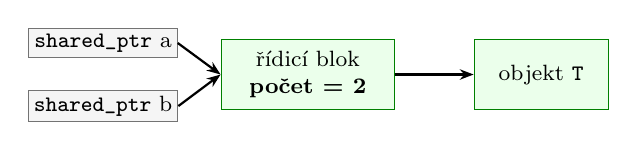
\begin{tikzpicture}[font=\footnotesize,node distance=5mm]
  \node[mem,minimum width=1.7cm] (sp1) {\texttt{shared\_ptr} a};
  \node[mem,minimum width=1.7cm,below=4mm of sp1] (sp2) {\texttt{shared\_ptr} b};
  \node[heapblk,minimum width=2.2cm,minimum height=9mm,align=center] (cb) at ($(sp1)!0.5!(sp2)+(2.6cm,0)$) {řídicí blok\\\textbf{počet = 2}};
  \node[heapblk,minimum width=1.7cm,minimum height=9mm,right=10mm of cb] (obj) {objekt \texttt{T}};
  \draw[ptr] (sp1.east) -- (cb.west);
  \draw[ptr] (sp2.east) -- (cb.west);
  \draw[ptr] (cb.east) -- (obj.west);
\end{tikzpicture}\\[2pt]
{\small (a) sdílené vlastnictví: oba ukazatele drží týž objekt, počet $=2$}
\end{minipage}\hfill
\begin{minipage}[t]{0.44\linewidth}\centering
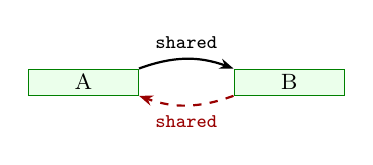
\begin{tikzpicture}[font=\footnotesize,node distance=8mm]
  \node[heapblk,minimum width=1.4cm] (A) {A};
  \node[heapblk,minimum width=1.4cm,right=12mm of A] (B) {B};
  \draw[ptr] (A.north east) to[bend left=20] node[above,font=\scriptsize]{\texttt{shared}} (B.north west);
  \draw[ptr,dashed,red!60!black] (B.south west) to[bend left=20] node[below,font=\scriptsize]{\texttt{shared}} (A.south east);
\end{tikzpicture}\\[2pt]
{\small (b) cyklus: počet nikdy neklesne na 0 $\Rightarrow$ únik; opravit jeden směr na \cd{weak_ptr}}
\end{minipage}
\end{center}
\obrpopis{Počítání referencí u \cd{shared_ptr}: řídicí blok eviduje, kolik vlastníků objekt drží (a); při zániku posledního (počet $\to 0$) se objekt uvolní. Vzájemný odkaz dvou objektů přes \cd{shared_ptr} (b) udržuje počet trvale kladný, takže se neuvolní nikdy (únik paměti) -- proto se jeden směr odkazu volí jako \cd{weak_ptr}, který počet nezvyšuje.}

\subsection{Správa paměti: C++ vs. spravovaná prostředí}

\begin{intuice}
Spravované jazyky (Java, C\#) mají \emph{garbage collector} (GC): běhové prostředí samo najde a uvolní objekty, na které už nevede žádný odkaz. Výhoda: programátor neřeší uvolňování. Nevýhody: nedeterministické pauzy, vyšší spotřeba paměti, pozdní uvolnění \emph{ne-paměťových} zdrojů (soubory, zámky) -- proto i ony zavádějí explicitní mechanismy (\texttt{using}, \texttt{try-with-resources}). C++ jde opačnou cestou: \textbf{deterministická} správa přes RAII a chytré ukazatele -- zdroj se uvolní v přesně daný okamžik (konec platnosti vlastníka), bez GC a jeho režie. Reference counting (\cd{shared_ptr}) je „lokální`` náhrada GC s přiznanou cenou a omezením (cykly).
\end{intuice}

\begin{csalt}[GC místo ručního životního cyklu]
Otázky, které kladou důraz na \emph{garbage collector}, \emph{finalizátory} nebo prostou správu paměti, jsou v~C\# přímočařejší: paměť uvolní GC, takže odpadá \emph{pravidlo pěti}, chytré ukazatele i ruční \cd{delete}. Ne-paměťové zdroje (soubor, zámek, spojení) se uklízejí \emph{deterministicky} přes rozhraní \cd{IDisposable} a příkaz \cd{using} -- to je protějšek RAII (sekce~4) a Javovského \texttt{try-with-resources}:
\begin{lstlisting}[style=cs]
using (var f = File.OpenText("a.txt")) { /* ... */ }   // Dispose() na konci bloku
\end{lstlisting}
\emph{Pozn.:} na rozdíl od RAII (úklid je automaticky v~destruktoru) je \cd{using} \emph{explicitní} a finalizátor \lstinline[style=cs]!~T()! volá GC nedeterministicky, takže se na něj pro včasné uvolnění zdrojů nelze spolehnout.
\end{csalt}

% ============================================================
\section{Vlákna a synchronizace}

\emph{Vlákno} (thread) je samostatný tok výpočtu uvnitř procesu; vlákna téhož procesu sdílejí paměť. C++ je reprezentuje objektem \cd{std::thread} (hlavička \texttt{<thread>}). Sdílení paměti přináší \emph{časově závislé chyby}, proti nimž slouží \emph{synchronizační prostředky}.

\subsection{Reprezentace vlákna a spuštění}

\begin{definice}[\texttt{std::thread}]
\cd{std::thread} je objekt spravující jedno běžící vlákno operačního systému. Konstruktor dostane \emph{volatelné} (funkci, lambdu, funktor) a jeho argumenty a vlákno \textbf{ihned spustí}. Vlákno je nutné před zánikem objektu buď \cd{join()} (počkat na jeho dokončení), nebo \cd{detach()} (osamostatnit). Zanikne-li \cd{std::thread} ještě \cd{joinable()}, zavolá se \cd{std::terminate}.
\end{definice}

\begin{lstlisting}[style=cpp]
#include <thread>
void prace(int id) { /* ... */ }

std::thread t1(prace, 1);                 // spustí vlákno s funkcí + argumentem
std::thread t2([]{ /* tělo */ });         // nebo s lambdou
unsigned n = std::thread::hardware_concurrency();  // počet HW vláken
t1.join();                                // počká na dokončení t1
t2.join();
\end{lstlisting}

\begin{poznamka}
Funkce vykonávaná vláknem se předá jako kterékoli volatelné; argumenty se vláknu \emph{kopírují} (pro předání odkazem je nutné \cd{std::ref}). Výjimka vyhozená ve vlákně se v jiném vlákně přímo chytit nedá -- nezachytí-li ji vlákno samo, volá se \cd{std::terminate}. Přenést ji do jiného vlákna lze jen explicitně (\cd{std::exception_ptr}, případně ji přenese \cd{std::async}/\cd{std::future} při volání \cd{get()}).
\end{poznamka}

\subsection{Časově závislé chyby a kritická sekce}

\begin{definice}[Souběh / datový závod, kritická sekce]
\emph{Časově závislá chyba} (race condition) nastává, když výsledek závisí na nedeterministickém prokládání vláken plánovačem OS. \emph{Datový závod} je její typický případ: dvě vlákna přistupují ke sdílené proměnné a aspoň jedno zapisuje, bez synchronizace. \emph{Kritická sekce} je úsek kódu, který smí v jeden okamžik provádět nejvýš jedno vlákno.
\end{definice}

\begin{lstlisting}[style=cpp]
int citac = 0;                 // sdílený stav
void inc() { ++citac; }        // ++ NENÍ atomické: načti, zvyš, ulož
// Dvě vlákna volají inc() 1000x. Bez synchronizace může výsledek být < 2000:
// obě načtou stejnou hodnotu, obě uloží +1, jeden zápis se "ztratí".
\end{lstlisting}

\begin{intuice}
Operace \cd{++citac} se přeloží na tři kroky (čti, zvyš, zapiš). Proloží-li plánovač dvě vlákna mezi čtením a zápisem, oba načtou např.\ $5$, oba zapíšou $6$ -- jeden přírůstek zmizí. Proto je výsledek nedeterministický a může být menší, než by měl být (v C++ je datový závod navíc nedefinované chování).
\end{intuice}

\subsection{Synchronizační prostředky}

\begin{definice}[Mutex, \texttt{lock\_guard}]
\cd{std::mutex} (vzájemné vyloučení) zajistí, že kritickou sekci provádí nejvýš jedno vlákno: vlákno mutex \emph{zamkne} (\cd{lock}) a po dokončení \emph{odemkne} (\cd{unlock}). RAII obal \cd{std::lock_guard} zamkne v konstruktoru a \textbf{odemkne v destruktoru} -- nelze zapomenout odemknout ani při výjimce.
\end{definice}

\begin{lstlisting}[style=cpp]
std::mutex m;
int citac = 0;
void inc() {
    std::lock_guard<std::mutex> g(m);   // zamkne; odemkne se na konci bloku
    ++citac;                            // kritická sekce: jen jedno vlákno naráz
}
\end{lstlisting}

\begin{csalt}[lock místo mutex + lock\_guard]
C\# má pro kritickou sekci přímo příkaz \cd{lock}: zápis \lstinline[style=cs]!lock (zamek) { ++citac; }! zamkne objekt na dobu bloku a spolehlivě odemkne i při výjimce (přeloží se na \texttt{Monitor.Enter}/\texttt{Exit} v~\texttt{try/finally}). Je stručnější než dvojice \cd{std::mutex} $+$ \cd{std::lock_guard}, kterou ovšem v~podstatě jen zapouzdřuje. Vlákno se spustí přes \lstinline[style=cs]!new Thread(prace).Start()! nebo úlohou \lstinline[style=cs]!Task.Run(...)!; vyšší úroveň nabízí \cd{async}/\cd{await}.
\end{csalt}

\begin{poznamka}[Uváznutí a další prostředky]
\emph{Uváznutí} (deadlock) nastane, když dvě vlákna čekají navzájem na zámky, které drží to druhé. Pomáhá zamykat více mutexů \emph{najednou} přes \cd{std::scoped_lock} (zamkne je v bezpečném pořadí). Další prostředky: \cd{std::condition_variable} (vlákno čeká na podmínku a je probuzeno notifikací -- producent/konzument), \cd{std::atomic<T>} (operace bez zámku, např.\ atomický \cd{++}). Podrobnosti \emph{paměťového modelu} atomických operací jdou nad rámec požadavků okruhu.
\end{poznamka}

% ============================================================
\section{Implementace OO jazyků (tabulka virtuálních metod)}

Tato sekce ukazuje, \emph{jak} se objektové konstrukce realizují v paměti -- zvlášť dynamický polymorfismus přes \emph{tabulku virtuálních metod}.

\subsection{Reprezentace primitivních a složených typů}

\begin{poznamka}
\emph{Primitivní} typy mají pevnou velikost a v paměti leží přímo (bez hlavičky). \emph{Složený} objekt (\cd{struct}/\cd{class}) je v paměti \emph{posloupnost} svých datových položek v pořadí deklarace; mezi ně překladač vkládá \emph{výplň} (padding) kvůli zarovnání (alignment). Objekt odvozené třídy obsahuje \emph{podobjekt báze} (její položky) následovaný vlastními položkami. Třída \textbf{bez} virtuálních metod (a bez virtuálních bází) nemá v objektu žádnou skrytou režii -- proto C++ objekt může být stejně úsporný jako čisté \texttt{C}.
\end{poznamka}

\subsection{Tabulka virtuálních metod (vtable)}

\begin{definice}[vtable, vptr]
Má-li třída aspoň jednu virtuální metodu, překladač pro ni vytvoří \emph{tabulku virtuálních metod} (vtable) -- pole ukazatelů na konkrétní implementace virtuálních metod této třídy. Každý objekt takové třídy nese skrytý ukazatel \emph{vptr} na vtable své (nejodvozenější) třídy. Volání virtuální metody přes ukazatel/referenci pak proběhne nepřímo: \emph{dereferencuj vptr $\to$ najdi v tabulce položku metody $\to$ zavolej}.
\end{definice}

\begin{center}
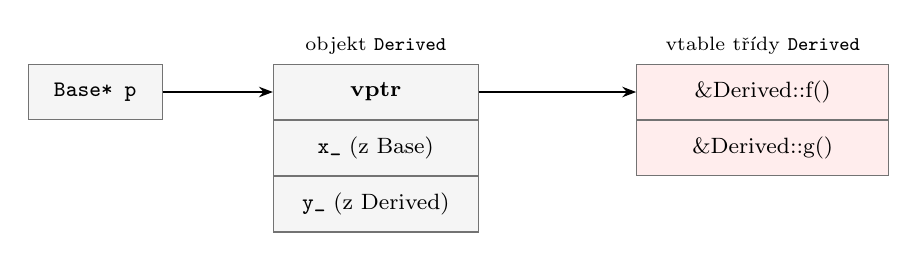
\begin{tikzpicture}[font=\footnotesize,node distance=0pt]
  % pointer
  \node[mem,minimum width=1.7cm,minimum height=7mm] (p) {\texttt{Base* p}};
  % object cells (vertical)
  \node[mem,minimum width=2.6cm,minimum height=7mm,right=14mm of p] (vptr) {\textbf{vptr}};
  \node[mem,minimum width=2.6cm,minimum height=7mm,below=0pt of vptr] (mx) {\texttt{x\_} (z Base)};
  \node[mem,minimum width=2.6cm,minimum height=7mm,below=0pt of mx] (my) {\texttt{y\_} (z Derived)};
  \node[anchor=south,font=\scriptsize] at (vptr.north) {objekt \texttt{Derived}};
  % vtable cells (vertical), to the right of vptr
  \node[mem,fill=red!7,minimum width=3.2cm,minimum height=7mm,right=20mm of vptr] (v0) {\&Derived::f()};
  \node[mem,fill=red!7,minimum width=3.2cm,minimum height=7mm,below=0pt of v0] (v1) {\&Derived::g()};
  \node[anchor=south,font=\scriptsize] at (v0.north) {vtable třídy \texttt{Derived}};
  % arrows
  \draw[ptr] (p.east) -- (vptr.west);
  \draw[ptr] (vptr.east) -- (v0.west);
\end{tikzpicture}
\obrpopis{Rozložení objektu \texttt{Derived} (báze \texttt{Base}): na začátku skrytý \textbf{vptr}, pak položky báze a potomka. vptr míří na vtable třídy \texttt{Derived}, kde jsou adresy skutečných implementací virtuálních metod. Volání \texttt{p->f()} přes \texttt{Base*}: přečti vptr, vyber položku \texttt{f}, zavolej \texttt{Derived::f} -- to je \emph{dynamický} výběr podle skutečného typu objektu, ne podle typu ukazatele.}
\end{center}

\begin{poznamka}
Cena dynamického polymorfismu = jedna nepřímost navíc (přes vtable) a skrytý vptr v objektu; proto se v C++ za virtuální metody „platí`` jen tam, kde se použijí. Vedle adres metod nese vtable i pomocné položky (zejména ukazatel na \texttt{type\_info} pro RTTI -- běhovou typovou informaci -- a \cd{dynamic_cast}), které ve skutečnosti leží \emph{před} adresami metod; pro princip je ale podstatné právě pole adres metod, na jehož začátek vptr ukazuje. U \emph{vícenásobné} dědičnosti má objekt více vptr (po jednom na každou polymorfní bázi); u \emph{virtuální} dědičnosti se navíc poloha sdílené báze zjišťuje přes uložené offsety. Konstrukce vtable se dělá automaticky; je to běžný způsob, jak objektové jazyky (C++, ale i Java/C\#) implementují virtuální volání.
\end{poznamka}

% ============================================================
\section{Nativní a interpretovaný běh, překlad a sestavení}

Poslední téma je „cesta od zdrojového kódu ke spuštěnému programu``: jak se C++ překládá a sestavuje a čím se to liší od interpretovaných / bytecode jazyků.

\subsection{Reprezentace programu, oddělený překlad}

\begin{definice}[Hlavička, překladová jednotka, deklarace vs. definice]
\emph{Hlavičkový soubor} (\texttt{.hpp}) obsahuje \emph{rozhraní} -- deklarace (co existuje); \emph{zdrojový soubor} (\texttt{.cpp}) obsahuje \emph{implementaci} -- definice (jak to funguje). \emph{Překladová jednotka} (translation unit) je jeden \texttt{.cpp} po vložení všech \cd{#include}. \emph{Oddělený překlad} znamená, že každá překladová jednotka se přeloží \textbf{nezávisle} na \emph{objektový soubor} (\texttt{.o}); změna jednoho \texttt{.cpp} nevyžaduje překlad ostatních.
\end{definice}

\begin{poznamka}
\emph{Deklarace} oznamuje existenci jména (smí jich být víc); \emph{definice} ho zavádí (\emph{One Definition Rule}, ODR: nejvýš jedna v celém programu; výjimkou jsou definice tříd, \cd{inline} funkce a šablony, jejichž shodná definice smí být v každé překladové jednotce). \cd{#include} je čistě textové vložení (preprocesorem). Šablony musí být celé v hlavičce (definice musí být viditelná v místě instanciace), proto nejdou oddělit do \texttt{.cpp}.
\end{poznamka}

\begin{center}
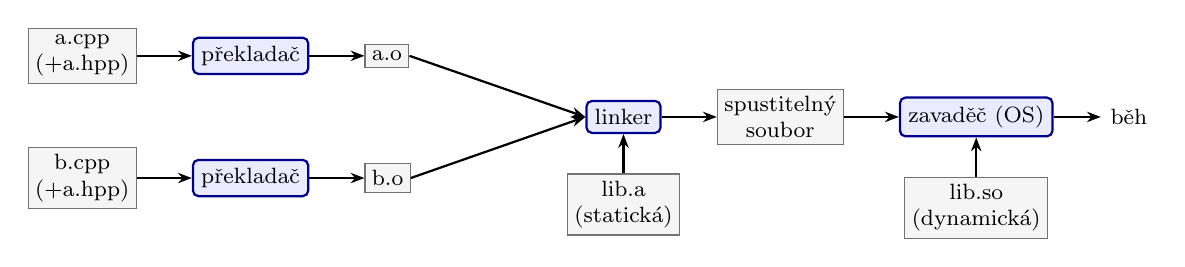
\begin{tikzpicture}[font=\footnotesize,node distance=5mm and 7mm,
   proc/.style={rectangle,rounded corners=2pt,draw=blue!55!black,fill=blue!8,thick,inner sep=3pt,align=center,font=\footnotesize},
   fil/.style={rectangle,draw=black!55,fill=black!4,inner sep=2.5pt,font=\footnotesize,align=center}]
  \node[fil] (acpp) {a.cpp\\(+a.hpp)};
  \node[proc,right=of acpp] (cc1) {překladač};
  \node[fil,right=of cc1] (ao) {a.o};
  \node[fil,below=8mm of acpp] (bcpp) {b.cpp\\(+a.hpp)};
  \node[proc,right=of bcpp] (cc2) {překladač};
  \node[fil,right=of cc2] (bo) {b.o};
  \node[proc] (link) at ($(ao)!0.5!(bo)+(3.0cm,0)$) {linker};
  \node[fil,right=of link] (exe) {spustitelný\\soubor};
  \node[proc,right=of exe] (load) {zavaděč (OS)};
  \node[right=6mm of load] (run) {běh};
  \node[fil,below=5mm of link] (lib) {lib.a\\(statická)};
  \node[fil,below=5mm of load] (so) {lib.so\\(dynamická)};
  \draw[flow] (acpp)--(cc1); \draw[flow] (cc1)--(ao);
  \draw[flow] (bcpp)--(cc2); \draw[flow] (cc2)--(bo);
  \draw[flow] (ao.east) -- (link.west);
  \draw[flow] (bo.east) -- (link.west);
  \draw[flow] (lib.north) -- (link.south);
  \draw[flow] (link)--(exe); \draw[flow] (exe)--(load); \draw[flow] (load)--(run);
  \draw[flow] (so.north) -- (load.south);
\end{tikzpicture}
\obrpopis{Sestavení programu v C++: každá překladová jednotka (\texttt{a.cpp}, \texttt{b.cpp}) se přeloží \emph{nezávisle} na objektový soubor (\texttt{.o}). \emph{Linker} slije objektové soubory a \emph{statické} knihovny (\texttt{.a}) do spustitelného souboru. \emph{Zavaděč} operačního systému ho při spuštění nahraje do paměti a připojí \emph{dynamické} (sdílené) knihovny (\texttt{.so}).}
\end{center}

\subsection{Statické a dynamické knihovny}

\begin{poznamka}
\emph{Statická} knihovna (\texttt{.a} / \texttt{.lib}) se \textbf{při linkování zkopíruje} (její potřebné části) do spustitelného souboru -- program je samostatný, ale větší a knihovnu nelze aktualizovat bez relinkování. \emph{Dynamická / sdílená} knihovna (\texttt{.so} / \texttt{.dll}) se připojí \textbf{až za běhu} zavaděčem -- spustitelný soubor je menší, jednu kopii kódu v paměti sdílí více procesů a knihovnu lze aktualizovat zvlášť (cenou je závislost na přítomnosti správné verze). Program si může sdílenou knihovnu načíst i sám za běhu (\texttt{dlopen} v~POSIX, \texttt{LoadLibrary} ve Windows) a vyhledat v~ní symboly podle jména -- tak fungují \emph{pluginy} (viz otázka jaro~2023).
\end{poznamka}

\subsection{Nativní vs. interpretovaný běh, AOT vs. JIT}

\begin{definice}[Nativní/AOT vs. interpretovaný/bytecode/JIT]
\emph{C++ je překládán dopředně} (AOT, ahead-of-time) přímo do \emph{nativního strojového kódu} cílové platformy; za běhu nepotřebuje interpret ani překladač. Naproti tomu jazyky jako Java či C\# se překládají do \emph{bytecode} (mezikódu: \texttt{.class} u~Javy, IL u~.NET), který běží ve \emph{virtuálním stroji} (JVM, .NET CLR): ten ho \emph{interpretuje}, nebo \emph{překládá za běhu} (JIT, just-in-time) na nativní kód. JVM typicky kombinuje obojí (interpretuje a JIT překládá jen často prováděná místa), .NET CLR metody před prvním voláním JIT překládá. I pro tyto jazyky existuje AOT překlad do nativního kódu (např.\ GraalVM Native Image, .NET Native AOT); AOT tedy není vlastnost jazyka, ale způsobu jeho implementace.
\end{definice}

\begin{center}
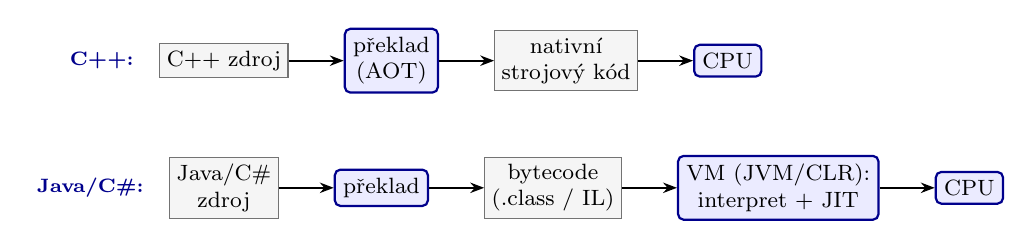
\begin{tikzpicture}[font=\footnotesize,node distance=4mm and 7mm,
   proc/.style={rectangle,rounded corners=2pt,draw=blue!55!black,fill=blue!8,thick,inner sep=3pt,align=center,font=\footnotesize},
   fil/.style={rectangle,draw=black!55,fill=black!4,inner sep=2.5pt,font=\footnotesize,align=center}]
  % AOT row
  \node[fil] (csrc) {C++ zdroj};
  \node[proc,right=of csrc] (caot) {překlad\\(AOT)};
  \node[fil,right=of caot] (nat) {nativní\\strojový kód};
  \node[proc,right=of nat] (cpu1) {CPU};
  \draw[flow] (csrc)--(caot); \draw[flow] (caot)--(nat); \draw[flow] (nat)--(cpu1);
  \node[left=2mm of csrc,font=\scriptsize\bfseries,align=right,text=blue!55!black] {C++:};
  % JIT row
  \node[fil,below=10mm of csrc] (jsrc) {Java/C\#\\zdroj};
  \node[proc,right=of jsrc] (jc) {překlad};
  \node[fil,right=of jc] (bc) {bytecode\\(.class / IL)};
  \node[proc,right=of bc] (vm) {VM (JVM/CLR):\\interpret + JIT};
  \node[proc,right=of vm] (cpu2) {CPU};
  \draw[flow] (jsrc)--(jc); \draw[flow] (jc)--(bc); \draw[flow] (bc)--(vm); \draw[flow] (vm)--(cpu2);
  \node[left=2mm of jsrc,font=\scriptsize\bfseries,align=right,text=blue!55!black] {Java/C\#:};
\end{tikzpicture}
\obrpopis{Nativní (AOT) běh C++ vs. bytecode/JIT běh spravovaných jazyků. C++ se přeloží dopředně na nativní strojový kód, který procesor vykonává přímo. Java/C\# se přeloží na přenositelný bytecode, jejž virtuální stroj za běhu interpretuje nebo JIT-překládá na nativní kód. AOT dává předvídatelný výkon a žádnou běhovou režii navíc; JIT umožňuje přenositelnost a optimalizace podle skutečného běhu za cenu rozběhové latence a běhového prostředí.}
\end{center}

\subsection{Běhové prostředí a vazba na OS}

\begin{poznamka}
Spustitelný soubor zavádí do paměti \emph{zavaděč} operačního systému, předá řízení startovacímu kódu běhového prostředí (inicializace, konstruktory globálních objektů) a ten zavolá \cd{main}. \emph{Běhové prostředí} (runtime) C++ je minimální (na rozdíl od JVM/CLR) -- v omezených prostředích (embedded, jádro OS) může program běžet skoro bez něj. C/C++ je proto jazykem operačních systémů a běhových knihoven jiných jazyků.
\end{poznamka}

\begin{priklad}[SZZ léto 2022 č.~2: Překlad konstrukcí vyššího jazyka]
\szzotazka{léto 2022}{2}{Překlad konstrukcí vyššího jazyka}\par

\textbf{Zadání.}\par
Procesor inspirovaný MIPS má registry \texttt{\$R0}--\texttt{\$R31}
(\texttt{\$R0 = 0}) a \texttt{PC}; instrukce \texttt{LD reg=[mem]},
\texttt{ST [mem]=reg}, \texttt{ADD r1=r2,r3}, \texttt{J label},
\texttt{BEQ/BNE r1,r2,label} (skok při rovnosti / nerovnosti) a
\texttt{SLT r1=r2,r3} (\texttt{r1 = (r2 < r3)}). Dána je posloupnost:

\begin{lstlisting}[style=cpp,language=]
        LD  $r1=[q]   LD  $r2=[n]   LD  $r3=[inc]   J  lab1
lab2:   LD  $r4=[a]   LD  $r5=[b]   ADD $r4=$r4,$r1
        SLT $r5=$r5,$r4    BEQ $r5,$r0,lab3
        ST  [b]=$r4
lab3:   ADD $r1=$r1,$r3
lab1:   SLT $r4=$r1,$r2    BNE $r4,$r0,lab2
\end{lstlisting}
Úkoly: (1)~vybrat z~nabídnutých úryvků v~C ty, které posloupnosti odpovídají, a~připsat k~instrukcím čísla řádků odpovídajících příkazů;
(2)~jak se C kód změní, nahradíme-li \texttt{BEQ} za \texttt{BNE} (stejné operandy);
(3)~upravit posloupnost tak, aby realizovala podmínku rozšířenou o \texttt{\&\& i < b}.

\medskip
\textbf{Řešení.}\par
\textbf{(1)} Test cyklu \texttt{SLT \$r4=\$r1,\$r2} + \texttt{BNE \$r4,\$r0,lab2}
běží \emph{dokud} \texttt{i < n} (řídicí \texttt{i} je \texttt{\$r1}, start
\texttt{q}, krok \texttt{inc}). V~těle dá \texttt{SLT \$r5=\$r5,\$r4} hodnotu
\texttt{\$r5 = (b < a+i)} a \texttt{BEQ \$r5,\$r0,lab3} \emph{přeskočí} uložení,
když \texttt{\$r5 == 0}, tj. \texttt{a+i <= b}; \texttt{b = a+i} se tedy provede
právě když \texttt{a+i > b}. Posloupnost realizuje (a~odpovídají \emph{obě} tyto
nabízené varianty):
\begin{lstlisting}[style=cpp,language=C]
for (i=q; i<n; i+=inc) if (a+i > b) b = a+i;
// ekvivalentne:  i=q; while (i<n) { if (a+i > b) b = a+i; i += inc; }
\end{lstlisting}
Čísla řádků: načtení \texttt{q}, \texttt{n}, \texttt{inc}, skok \texttt{J lab1}, přičtení \texttt{inc} a~test \texttt{SLT}/\texttt{BNE} na konci patří k~hlavičce \texttt{for}; načtení \texttt{a}, \texttt{b}, součet, \texttt{SLT} a~\texttt{BEQ} k~\texttt{if}; \texttt{ST} k~přiřazení (u~varianty s~\texttt{while} obdobně, přehled je v~dokumentu \emph{Příklady otázek}).

\textbf{(2)} Záměna \texttt{BEQ}$\to$\texttt{BNE} obrátí podmínku skoku: přeskočení
nastane, když \texttt{\$r5 != 0} (tj. \texttt{a+i > b}), takže uložení proběhne
v~opačném případě. Podmínka se změní na \cd{if (a+i <= b) b = a+i;}.

\textbf{(3)} Rozšíření o \texttt{\&\& i < b}: před \texttt{ST [b]=\$r4} vložíme
druhý test (\texttt{i < b}); když neplatí, přeskočíme uložení na \texttt{lab3}:
\begin{lstlisting}[style=cpp,language=]
        SLT $r5=$r5,$r4        ; r5 = (b < a+i)
        BEQ $r5,$r0,lab3       ; preskoc, kdyz a+i <= b
        LD  $r6=[b]            ; pridany test i < b
        SLT $r6=$r1,$r6        ; r6 = (i < b)
        BEQ $r6,$r0,lab3       ; preskoc, kdyz i < b neplati
        ST  [b]=$r4            ; ulozi se jen kdyz a+i > b AND i < b
\end{lstlisting}
\end{priklad}

% ============================================================
\section*{Shrnutí}
\addcontentsline{toc}{section}{Shrnutí}

\begin{poznamka}
\textbf{Klíčové pojmy a fakta (přehled k~SZZ).} Hlavní témata okruhu I3: OO návrh a rozhraní, C++ idiomy (RAII, šablony, chytré ukazatele), implementace runtime (vtable, překlad). Zkratky: UB = undefined behaviour; RAII = Resource Acquisition Is Initialization; ODR = One Definition Rule.

\smallskip
\emph{Abstrakce, zapouzdření, polymorfismus, dědičnost.}
\begin{itemize}
  \item Abstrakce = skrytí implementace za rozhraní; zapouzdření = řízený přístup přes \cd{public}/\cd{protected}/\cd{private}. Dědičnost IS-A (veřejná); potomek rozšiřuje a může překrývat.
  \item Virtuální metoda (\cd{virtual}): dynamický dispatch za běhu přes vptr. Nevirtuální: statická vazba za překladu. Čistě virtuální (\cd{= 0}): potomek musí překrýt; třída s aspoň jednou \cd{= 0} = abstraktní (nelze instanciovat) = C++ „rozhraní".
  \item Polymorfní báze \textbf{musí mít virtuální destruktor}; jinak \cd{delete} přes ukazatel na bázi = UB.
  \item \textbf{Přetěžování} (overloading): stejné jméno, různé signatury -- volba staticky za překladu. \textbf{Překrývání} (overriding): \cd{virtual} + \cd{override} -- volba dynamicky za běhu. \cd{override} zachytí překlep v~signatuře.
  \item Pozor na \textbf{slicing}: přiřazení polymorfního objektu \emph{hodnotou} ořízne potomkovy členy.
  \item \emph{SZZ vzory:} \texttt{IFilter}/\texttt{IImageFormat} (bitmapový editor, jaro~2023); \texttt{IGraph}/\texttt{IVertex}/\texttt{IEdge} (podzim~2022); \texttt{Matrix} (jaro~2025); hierarchie \texttt{Element}/\texttt{Type}/\texttt{Method}/\texttt{Field} (podzim~2024).
\end{itemize}

\smallskip
\emph{Vícenásobná dědičnost, virtuální dědičnost, rozhraní.}
\begin{itemize}
  \item Diamantový problém: dvě kopie báze S (přes R, W) $\to$ dvojznačnost přístupu a redundantní data.
  \item Virtuální dědičnost (\texttt{class R : public virtual S}): jedna sdílená instance S.
  \item C++ nemá klíčové slovo \texttt{interface}; „rozhraní" = abstraktní třída (čistě virtuální metody + virtuální destruktor, žádné datové položky).
  \item Vhodné použití: IS-A $\to$ dědičnost; HAS-A $\to$ \textbf{kompozice} (upřednostnit); obecný kontrakt $\to$ abstraktní třída.
\end{itemize}

\smallskip
\emph{Primitivní a složené typy; ukazatele, reference, \texttt{const}.}
\begin{itemize}
  \item Číselné: \cd{int}/\cd{long}/\cd{float}/\cd{double}/\cd{bool}/\cd{char}; \cd{enum class}: typově bezpečný výčet (nevzniká implicitní převod na \cd{int}).
  \item Ukazatel \cd{T*}: může být \cd{nullptr}, lze rebindovat, aritmetika. Reference \cd{T&}: alias, nesmí být null, nelze rebindovat (může ale „viset``, zanikne-li odkazovaný objekt dřív než reference).
  \item \cd{const T&}: přijme dočasný i pojmenovaný. \cd{T&&}: r-value reference; základ pro přesun bez kopírování (move semantics).
  \item \cd{const} na metodě: garantuje nemodifikaci \cd{*this} (kromě \cd{mutable} položek). Vlastník vs.\ pozorovatel: \cd{unique_ptr}/\cd{shared_ptr} vlastní; holý \cd{T*} nebo reference pozoruje (nesmí přežít vlastníka).
\end{itemize}

\smallskip
\emph{Generické typy a statický polymorfismus.}
\begin{itemize}
  \item Šablony (templates): instanciace za překladu pro každý použitý typ; bez běhové režie. Požadavky na typ jsou implicitní (duck typing -- chybějící operátor/metoda = chyba za překladu).
  \item Specializace: úplná funguje u~šablon funkcí i~tříd; částečná \textbf{jen u~šablon tříd} (ne u~šablon funkcí).
  \item Statický polymorfismus (šablony) vs.\ dynamický (virtuální metody, vtable): statický = nulová nepřímost za běhu; dynamický = heterogenní kolekce přes ukazatele/reference na bázi.
  \item \cd{std::type_index}: klíč odvozený od RTTI (\cd{typeid}); klíčování typů v~mapě za běhu -- viz SZZ léto~2023 (\texttt{unordered\_map<type\_index,~unique\_ptr<Component>>}).
\end{itemize}

\smallskip
\emph{Typy reprezentující funkce; lambda, funkcionální rozhraní.}
\begin{itemize}
  \item Ukazatel na funkci \cd{R(*)(Args...)}: nejjednodušší; jen prosté funkce (ne lambdy se stavem).
  \item Funktor (třída s~\cd{operator()}): nese stav; základ, z~něhož kompilátor generuje lambdu.
  \item Lambda: \lstinline[style=cpp]![capture](params){body}! = anonymní funktor; \texttt{[=]} zachytí vše použité hodnotou; \texttt{[\&]} referencí; \texttt{[this]} ukazatel na objekt.
  \item \cd{std::function<R(Args...)>}: type erasure (typ volatelného se „vymaže``) -- přijme ukazatel, funktor i~lambdu; mírná běhová režie.
  \item \emph{SZZ podzim~2024:} průchod strukturou typu = vzor Visitor (\texttt{accept}/\texttt{visit}, dvojitá dispatch); operace = konkrétní návštěvník. Alternativy: operace jako lambda/\cd{std::function}, nebo \cd{std::variant} elementů + \cd{std::visit}.
\end{itemize}

\smallskip
\emph{RAII a výjimky.}
\begin{itemize}
  \item RAII: zdroj (soubor, mutex, paměť) = životnost objektu; konstruktor získá, destruktor uvolní. Správa funguje i~při výjimce. Nahrazuje \texttt{finally} z~Javy/C\#.
  \item Výjimky: \cd{throw}/\cd{try}/\cd{catch}, hierarchie \cd{std::exception}. Odvíjení zásobníku (stack unwinding) při výjimce volá destruktory všech lokálních objektů ve všech rámcích na cestě.
  \item Záruky: \emph{basic} (invariant zachován, žádný únik), \emph{strong} (commit-or-rollback), \emph{nothrow}. Destruktor by \textbf{nikdy} neměl házet (\cd{noexcept} od C++11 implicitně).
  \item \emph{SZZ jaro~2023:} \cd{unique_ptr<IFilter>} a \cd{unique_ptr<IImageFormat>} = RAII pro polymorfní objekty; \cd{std::function} jako Factory pro formáty načítané za běhu z~pluginu (.dll).
\end{itemize}

\smallskip
\emph{Životní cyklus a správa paměti.}
\begin{itemize}
  \item Alokace: statická (\cd{static}/globální), zásobník (lokální proměnné), halda (\cd{new}/\cd{delete}, lépe \cd{make_unique}/\cd{make_shared}).
  \item Pořadí init: báze $\to$ datové položky $\to$ tělo konstruktoru; destrukce přesně opačně. Položky inicializuje inicializační seznam (ne tělo konstruktoru); pořadí určuje pořadí deklarace, ne pořadí v seznamu.
  \item \textbf{Pravidlo pěti}: vlastní-li třída zdroj, definuj (nebo \cd{= delete}) destruktor, kopírovací konstruktor, kopírovací přiřazení, přesouvací konstruktor, přesouvací přiřazení. \textbf{Pravidlo nuly}: spolehni se na RAII členy, nic nedefinuj.
  \item \cd{unique_ptr}: exkluzivní vlastnictví (move-only). \cd{shared_ptr}: sdílené vlastnictví + ref-count. Cyklus \cd{shared_ptr} $\Rightarrow$ únik $\to$ \cd{weak_ptr} (nezvyšuje počet).
  \item C++ nemá GC: deterministická správa, destruktor volán na konci životnosti. Java/C\#: GC nedeterministický; finalizátor (\texttt{Finalize}) není totéž co destruktor.
\end{itemize}

\smallskip
\emph{Vlákna a synchronizace.}
\begin{itemize}
  \item \cd{std::thread(f, args...)}: spustí \cd{f} v~novém OS vlákně; \cd{join()} čeká na dokončení; \cd{detach()} odpojí (vlákno běží dál, nelze joinovat).
  \item Race condition: paralelní neatomická čtení-modifikace-zápis (neatomické \cd{++}) $\to$ nedeterministický výsledek; datový závod (data race) je v~C++ UB.
  \item Kritická sekce: \cd{std::mutex} + \cd{lock_guard} (RAII -- zamkne při vzniku, odemkne při destrukci). Deadlock = kruhové čekání na zámky. \cd{std::atomic<T>}: atomické operace bez mutexu.
  \item \cd{std::condition_variable}: čekání na podmínku (vlákno čeká, probuzeno notifikací -- vzor producent/konzument); musí být doprovázena mutexem.
\end{itemize}

\smallskip
\emph{Implementace OO (vtable, vptr, RTTI).}
\begin{itemize}
  \item Objekt = posloupnost položek (nejdříve báze, pak potomkovy) + skrytý \textbf{vptr} na začátku (u~polymorfní třídy).
  \item vtable = statické pole adres virtuálních metod třídy; vptr ukazuje na vtable; virtuální volání = dereference vptr + nepřímý skok.
  \item RTTI (Runtime Type Information) leží ve vtable před adresami metod (Itanium ABI: g++, clang); \cd{dynamic_cast} a \cd{typeid} přistupují přes RTTI.
  \item \cd{dynamic_cast<D*>(p)}: za běhu ověří RTTI; vrátí \cd{nullptr} při selhání (pro reference hodí \cd{bad_cast}). Vyžaduje polymorfní hierarchii (aspoň jedna \cd{virtual}).
\end{itemize}

\smallskip
\emph{Překlad, sestavení, AOT vs.\ JIT.}
\begin{itemize}
  \item Pipeline: preprocesor (\texttt{\#include}, \texttt{\#define}) $\to$ kompilátor (\texttt{.cpp} $\to$ \texttt{.o}) $\to$ linker (\texttt{.o} + knihovny $\to$ spustitelný) $\to$ zavaděč OS (+ dynamické knihovny).
  \item Statická knihovna (\texttt{.a}/\texttt{.lib}): kód se zkopíruje do exe (větší, soběstačný). Dynamická (\texttt{.so}/\texttt{.dll}): sdílená za běhu; lze dodat jako plugin za~běhu -- viz SZZ jaro~2023 (formáty obrázků jako \texttt{.dll} pluginy).
  \item ODR: každý symbol smí mít nejvýš jednu definici v~programu. Třídy, \cd{inline} funkce a šablony smějí být v~hlavičce (vícenásobné definice se sloučí).
  \item C++ = nativní/AOT: \texttt{.cpp} $\to$ strojový kód; žádný interpret ani GC. Java/C\# = bytecode (\texttt{.class}/IL) + VM (JVM/CLR) + JIT (přeloží kód za běhu; JVM hlavně často prováděná místa); AOT je i~u~nich možný (GraalVM, .NET Native AOT). AOT výhody: deterministická latence, žádný warmup; JIT výhody: portabilita, run-time optimalizace dle dat.
\end{itemize}

\smallskip
\emph{Kdy je lehčí C\# -- viz fialové boxy v~textu.}
\begin{itemize}
  \item \emph{Rozhraní:} klíčové slovo \texttt{interface} místo abstraktní třídy s~čistě virtuálními metodami.
  \item \emph{Vícenásobná dědičnost:} C\# ji nemá $\Rightarrow$ žádný diamantový problém; jedna třídní báze + libovolně rozhraní.
  \item \emph{Visitor:} \texttt{switch} se vzory typů (pattern matching) místo \texttt{accept}/\texttt{visit} -- viz SZZ podzim~2024.
  \item \emph{Správa paměti:} GC, žádné pravidlo pěti; \texttt{using}/\texttt{IDisposable} pro deterministické uvolnění zdrojů.
  \item \emph{Kritická sekce:} příkaz \texttt{lock(obj)}\,\{\dots\} místo \cd{mutex} + \cd{lock_guard}.
\end{itemize}
\end{poznamka}

\section*{Zdroje}
\addcontentsline{toc}{section}{Zdroje}

{\raggedright
\begin{itemize}
  \item D.~Bednárek: \emph{Programování v~C++} (NPRG041), přednáškové slidy, MFF UK, 2025/26 (primární zdroj výkladu: ukazatele a~reference, copy/move, chytré ukazatele, šablony, lambdy, dědičnost a~vtable, výjimky, překlad a~modularita).\\ \url{https://teaching.mff.cuni.cz/nprg041-web/}
  \item D.~Bednárek: \emph{Pokročilé programování v~C++} (NPRG051), přednáškové slidy, MFF UK, 2025/26 (bezpečnost vůči výjimkám, šablony do hloubky, vlákna a~synchronizace, atomické operace).\\ \url{https://teaching.mff.cuni.cz/nprg051-web/}
  \item \emph{cppreference.com}: referenční příručka jazyka C++ a~standardní knihovny (ověření sémantiky jazykových konstrukcí a~knihovních tříd).\\ \url{https://en.cppreference.com/w/}
  \item \emph{Itanium C++ ABI}: specifikace binárního rozhraní používaného překladači g++ a~clang (rozložení objektů a~tabulek virtuálních metod).\\ \url{https://itanium-cxx-abi.github.io/cxx-abi/abi.html}
  \item Microsoft: \emph{C\# documentation} (Microsoft Learn), dokumentace jazyka C\# (rámečky \emph{Lehčí v~C\#}).\\ \url{https://learn.microsoft.com/en-us/dotnet/csharp/}
  \item MFF UK: požadavky ke státní závěrečné zkoušce (Informatika, Bc.) a~zadání otázek z~minulých termínů.\\ \url{https://www.mff.cuni.cz/cs/studenti/bakalarske-studium/statni-zaverecne-zkousky/bakalarske-statni-zkousky-studijniho-programu-informatika}
\end{itemize}
\par}

\end{document}
